
\section{Two-term solution of the Boltzmann equation using BOLSIG+}

Electron impact involves the collision of an electron with (in this case neutral) atoms or molecules. If such an event takes place, this can lead to ionization, excited states and/or electron attachment processes. Also of interest are properties derived from an electron impact process such as the reduced electric field as a function of electron energy, and derived transport coefficients and reaction rates. To compute these properties it is necessary to first obtain the electron energy distribution function (EEDF), which under the conditions of a weakly-ionized plasma cannot be assumed to follow a Maxwellian distribution. To this end, the Boltzmann solver BOLSIG+ is used to obtain such distribution function and all derived transport and rate coefficients. This solver takes as input the cross-sections in $\rm m^2$ given as a function of the energy in eV and obtains the EEDF using a two-term approximation to this distribution.

\subsection{Settings: Physics}

The following parameters are selected in the BOLSIG+ interface:

\begin{itemize}
\item[1.]{AC field: NO}
\item[2.]{$E\times B$ field: NO}
\item[3.]{Superelastics: YES}
\item[4.]{electron-electron collisions: NO}
\item[5.]{electron-ion collisions: NO}
\item[6.]{Gas/excited states temperature: 300 K}
\end{itemize}
Changes to the latter 3 paramaters do not alter the results for $E/N$ vs electron temperature for the mixtures considered herein.

\subsection{Settings: Numerics}

The number of energy intervals is set to 200 with Automatic Grid type. All remaining convergence settings are kept to defaults.

\subsection{Settings: Advanced}

The following parameters are selected in the BOLSIG+ interface:

\begin{itemize}
\item[1.]{Include electron-neutral effects on Coulomb logarithm : YES}
\item[2.]{Ion charge parameter Z: 1.0}
\item[3.]{Ion-neutral mass ratio: 1.0}
\end{itemize}
All remaining parameters are kept to the default value.

\section{Reduced electric field vs electron temperature for various electron-neutral mixtures}

The electron energy range in which BOLSIG+ results are valid depend on the energy range of the corresponding cross-section data. Here, only the converged runs are kept, and any results extrapolated by BOLSIG+ are discarded. For higher electron temperatures for which there is no BOLSIG+ solution, the data is extrapolated by placing a spline control point for an electron temperature of $5\cdot10^6$ K, and a corresponding $E/N$ value that reflects the trend of the converged BOLSIG+ results. This last control point can be be modified to get the desired accuracy at very high temperatures. Results for several mixtures are shown below.

%
\subsection{Atomic hydrogen ($\rm H$)}

All the processes involving cross-sections used in the BOLSIG+ calculation are given in Table \ref{tab:tableH}. The reduced electric field results are shown in Fig. \ref{fig:electronimpact_H}.

\begin{table*}[!htbp]
  \center\fontsizetable
  \begin{threeparttable}
    \tablecaption{$\rm H$ electron impact processes with available cross-section data.}
    \label{tab:tableH}
    \fontsizetable
    \begin{tabular*}{\textwidth}{l@{\extracolsep{\fill}}llll}
    \toprule
    {no.}  & {process} & {type} &  {eV range}  &  {ref.} \\
    \midrule
      1 & $\rm e^- + H \rightarrow H^+ + e^- + e^-$  &  ionization  &  13.6-800  &  \cite{lxc:2024:morgan} \\ 
        \midrule
      2 & $\rm e^- + H \rightarrow e^- + H$  &  momentum transfer   &  0-1000  & \cite{lxc:2024:morgan}\\  
        \midrule
      3 & $\rm e^- + H \rightarrow e^- + H(2p)$  &  excitation   &  10.2-1000  & \cite{lxc:2024:morgan}\\ 
      4 & $\rm e^- + H \rightarrow e^- + H(2s)$  &  excitation   &  10.2-1000  & \cite{lxc:2024:morgan}\\ 

    \bottomrule
    \end{tabular*}
   \end{threeparttable}
\end{table*}

\begin{figure}[!htbp]
\subfigure[]{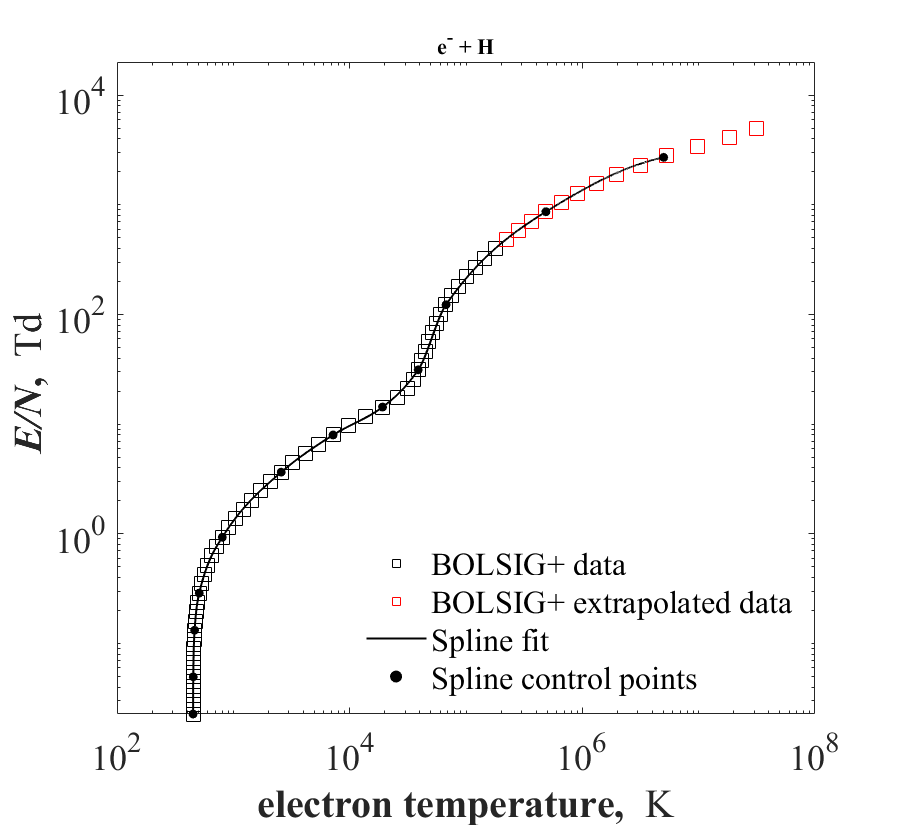
\includegraphics[width=0.99\linewidth, angle=0.0,scale=0.49]{electronimpact_figs/electronimpact_figureH.png}}
\subfigure[]{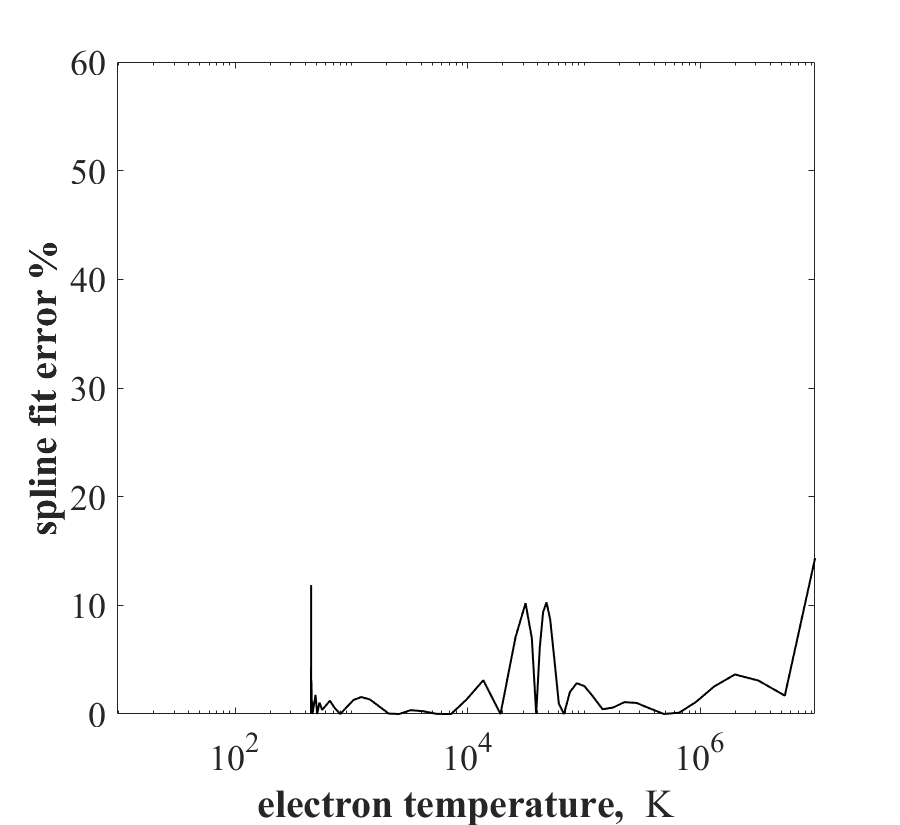
\includegraphics[width=0.99\linewidth, angle=0.0,scale=0.49]{electronimpact_figs/electronimpact_figureH_error.png}}
\caption{$E/N$ results for $\rm H$, showing (a) reduced electric field as a function of the electron temperature and (b) error percentage when fitting a cubic spline through BOLSIG+ data. The electron impact cross-sectional data used in the BOLSIG+ calculation is sourced from the Morgan database, Ref.\ \cite{lxc:2024:morgan}.}
\label{fig:electronimpact_H}
\end{figure}

%
\subsection{Hydrogen ($\rm H_2$)}

All the processes involving cross-sections used in the BOLSIG+ calculation are given in Table \ref{tab:tableH2}. The reduced electric field results are shown in Fig. \ref{fig:electronimpact_H2}.

\begin{table*}[!htbp]
  \center\fontsizetable
  \begin{threeparttable}
    \tablecaption{$\rm H_2$ electron impact processes with available cross-section data.}
    \label{tab:tableH2}
    \fontsizetable
    \begin{tabular*}{\textwidth}{l@{\extracolsep{\fill}}llll}
    \toprule
    {no.}  & {process} & {type} &  {eV range}  &  {ref.} \\
    \midrule
      1 & $\rm e^- + H_2 \rightarrow H_2^+ + e^- + e^-$  &  ionization  &  13.6-800  &  \cite{lxc:2024:morgan} \\ 
        \midrule
      2 & $\rm e^- + H_2 \rightarrow e^- + H_2$  &  momentum transfer   &  0-1000  & \cite{lxc:2024:morgan}\\  
        \midrule
      3 & $\rm e^- + H_2 \rightarrow e^- + H_2(00\rightarrow 20)$  &  rotational excitation   &  0.044-1000  & \cite{lxc:2024:morgan}\\ 
      4 & $\rm e^- + H_2 \rightarrow e^- + H_2(10\rightarrow 30)$  &  rotational excitation   &  0.079-1000  & \cite{lxc:2024:morgan}\\ 
              \midrule
      5 & $\rm e^- + H_2 \rightarrow e^- + H_2$$(\nu_1)$  &  vibrational excitation   &  0.516-1000  & \cite{lxc:2024:morgan}\\
      6 & $\rm e^- + H_2 \rightarrow e^- + H_2$$(\nu_2)$  &  vibrational excitation   &  1.000-1000  & \cite{lxc:2024:morgan}\\
      7 & $\rm e^- + H_2 \rightarrow e^- + H_2$$(\nu_3)$  &  vibrational excitation   &  1.500-1000  & \cite{lxc:2024:morgan}\\
                    \midrule
      8 & $\rm e^- + H_2 \rightarrow e^- + H_2$$(B^3\Sigma)$  &  electronic excitation   &  8.900-1000  & \cite{lxc:2024:morgan}\\
      9 & $\rm e^- + H_2 \rightarrow e^- + H_2$$(B^1\Sigma)$  &  electronic excitation   &  11.30-1000  & \cite{lxc:2024:morgan}\\
      10 & $\rm e^- + H_2 \rightarrow e^- + H_2$$(C^3\Pi)$  &  electronic excitation   &  11.75-1000  & \cite{lxc:2024:morgan}\\
      11 & $\rm e^- + H_2 \rightarrow e^- + H_2$$(A^3\Sigma)$  &  electronic excitation   &  11.80-1000  & \cite{lxc:2024:morgan}\\
     12 & $\rm e^- + H_2 \rightarrow e^- + H_2$$(C^1\Pi)$  &  electronic excitation   &  12.40-1000  & \cite{lxc:2024:morgan}\\
     13 & $\rm e^- + H_2 \rightarrow e^- + H_2$$({}^1\Sigma)$  &  electronic excitation   &  13.86-1000  & \cite{lxc:2024:morgan}\\
     14 & $\rm e^- + H_2 \rightarrow e^- + H_2$$(D^3\Pi)$  &  electronic excitation   &  14.00-1000  & \cite{lxc:2024:morgan}\\
     15 & $\rm e^- + H_2 \rightarrow e^- + H_{2}^*$  &  excitation   &  15.00-1000  & \cite{lxc:2024:morgan}\\
     16 & $\rm e^- + H_2 \rightarrow e^- + H_2$(Rydberg)  &  excitation   &  15.20-1000  & \cite{lxc:2024:morgan}\\
     16 & $\rm e^- + H_2 \rightarrow e^- + H_{2}^*$  &  excitation   &  16.60-1000  & \cite{lxc:2024:morgan}\\
    \bottomrule
    \end{tabular*}
   \end{threeparttable}
\end{table*}

\begin{figure}[!htbp]
\centering
\subfigure[]{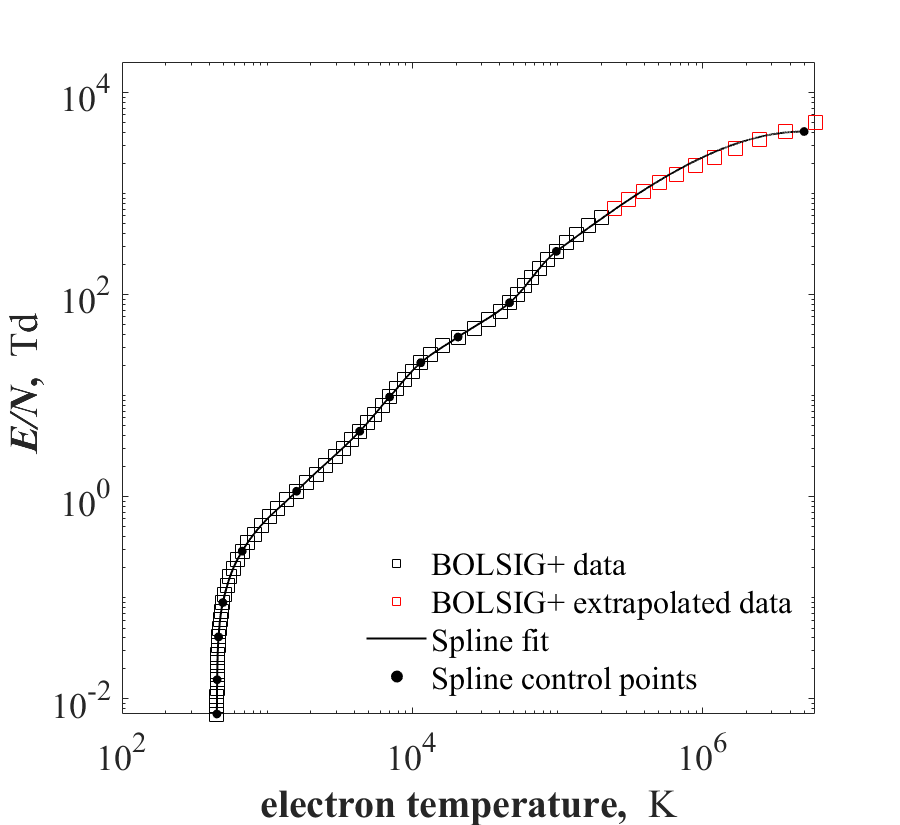
\includegraphics[width=0.99\linewidth, angle=0.0,scale=0.49]{electronimpact_figs/electronimpact_figureH2.png}}
\subfigure[]{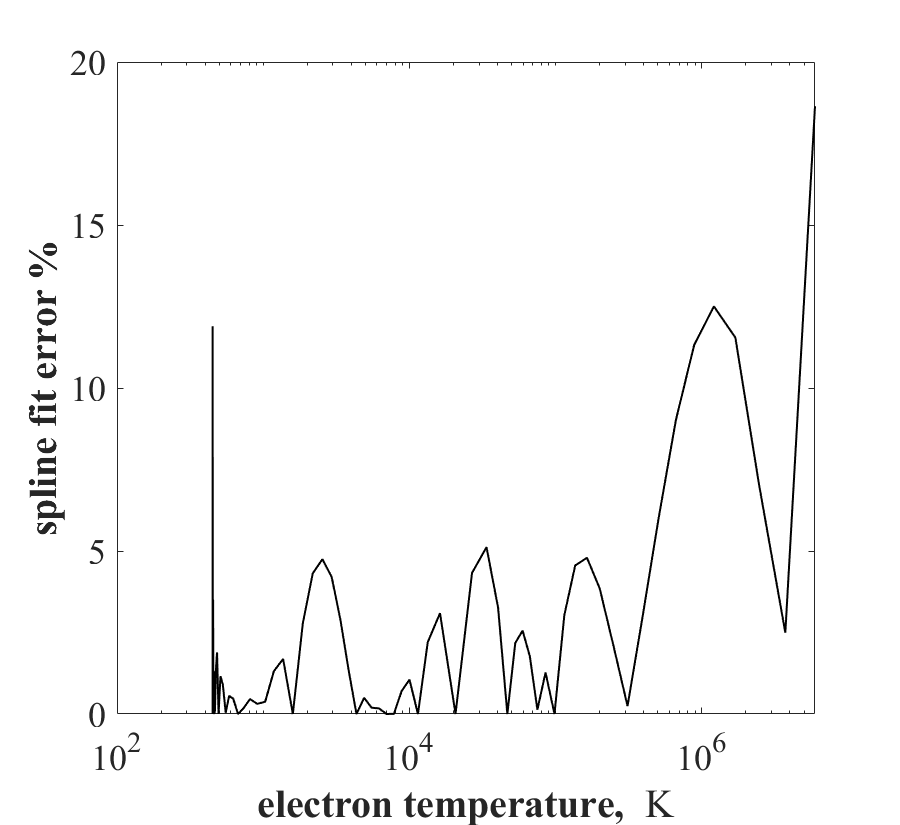
\includegraphics[width=0.99\linewidth, angle=0.0,scale=0.49]{electronimpact_figs/electronimpact_figureH2_error.png}}
\subfigure[]{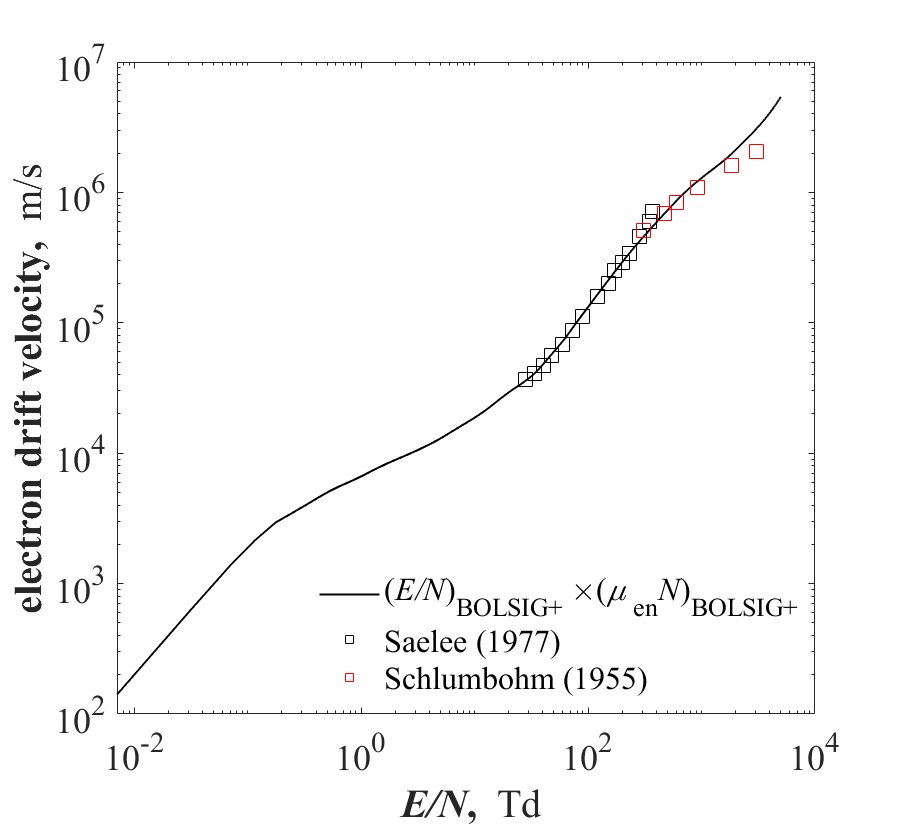
\includegraphics[width=0.99\linewidth, angle=0.0,scale=0.49]{electronimpact_figs/electronimpact_figureH2_drift.png}}
\caption{$E/N$ results for $\rm H_2$, showing (a) reduced electric field as a function of the electron temperature, (b) error percentage when fitting a cubic spline through BOLSIG+ data and c) drift velocity obtained from BOLSIG+ data as the product of the reduced electron mobility and the reduced electric field. The electron impact cross-sectional data used in the BOLSIG+ calculation is sourced from the Morgan database, Ref.\ \cite{lxc:2024:morgan}. Experimental drift velocity data is taken from Refs.\ \cite{thesis:1965:schlumbohm} and \cite{jop:1977:saelee}.}
\label{fig:electronimpact_H2}
\end{figure}
%

%
\subsection{Atomic nitrogen ($\rm N$)}

All the processes involving cross-sections used in the BOLSIG+ calculation are given in Table \ref{tab:tableN}. The reduced electric field results are shown in Fig. \ref{fig:electronimpact_4}.

\begin{table*}[!htbp]
  \center\fontsizetable
  \begin{threeparttable}
    \tablecaption{$\rm N$ electron impact processes with available cross-section data.}
    \label{tab:tableN}
    \fontsizetable
    \begin{tabular*}{\textwidth}{l@{\extracolsep{\fill}}llll}
    \toprule
    {no.}  & {process} & {type} &  {eV range}  &  {ref.} \\
    \midrule
      1 & $\rm e^- + N \rightarrow N^+ + e^- + e^-$  &  ionization   &  14.54-1000 &   \cite{lxc:2024:morgan} \\ 
      \midrule     
      2 & $\rm e^- + N \rightarrow e^- + N$  &  momentum transfer   &  0-23.1  & \cite{lxc:2024:morgan}\\   
      \midrule
      3 & $\rm e^- + N \rightarrow e^- + N(2p3)2D^0 $  &  electronic excitation   &  2.38-1000 & \cite{lxc:2024:morgan}\\ 
      4 & $\rm e^- + N \rightarrow e^- + N(2p3)2P^0 $  &  electronic excitation   &  3.58-1000 & \cite{lxc:2024:morgan}\\ 
      5 & $\rm e^- + N \rightarrow e^- + N(3p)4P $  &  electronic excitation   &  10.3-1000 & \cite{lxc:2024:morgan}\\ 
      6 & $\rm e^- + N \rightarrow e^- + N(2s2p4)4P $  &  electronic excitation   &  10.9-1000 & \cite{lxc:2024:morgan}\\ 
      7 & $\rm e^- + N \rightarrow e^- + N(3p) $  &  electronic excitation   &  11.84-1000 & \cite{lxc:2024:morgan}\\ 
      8 & $\rm e^- + N \rightarrow e^- + N(4s)4P $  &  electronic excitation   &  12.85-1000 & \cite{lxc:2024:morgan}\\ 
      9 & $\rm e^- + N \rightarrow e^- + N(3d) $  &  electronic excitation   &  13.0-1000 & \cite{lxc:2024:morgan}\\ 
      10 & $\rm e^- + N \rightarrow e^- + N(4p) $  &  electronic excitation   &  13.24-1000 & \cite{lxc:2024:morgan}\\ 
    \bottomrule
    \end{tabular*}
   \end{threeparttable}
\end{table*}

\begin{figure}[!htbp]
\subfigure[]{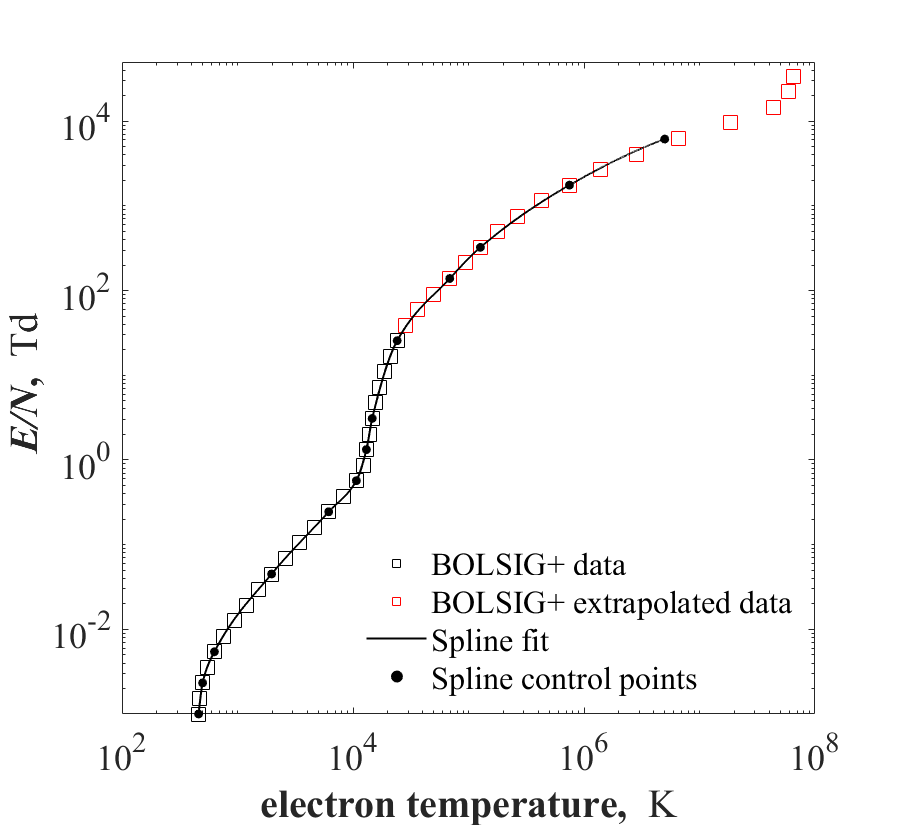
\includegraphics[width=0.99\linewidth, angle=0.0,scale=0.49]{electronimpact_figs/electronimpact_figure4.png}}
\subfigure[]{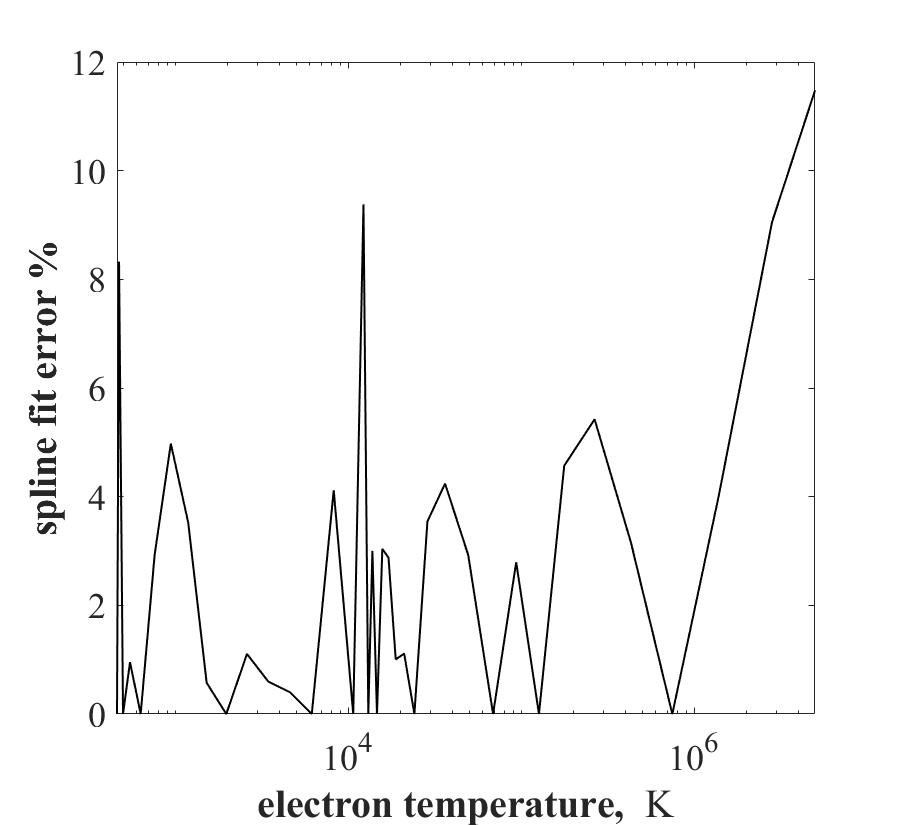
\includegraphics[width=0.99\linewidth, angle=0.0,scale=0.49]{electronimpact_figs/electronimpact_figure4_error.png}}
\caption{$E/N$ results for $\rm N$, showing (a) reduced electric field as a function of the electron temperature and (b) error percentage when fitting a cubic spline through BOLSIG+ data. The electron impact cross-sectional data used in the BOLSIG+ calculation is sourced from the Morgan database, Ref.\ \cite{lxc:2024:morgan}.}
\label{fig:electronimpact_4}
\end{figure}
%
\subsection{Atomic oxygen ($\rm O$)}

All the processes involving cross-sections used in the BOLSIG+ calculation are given in Table \ref{tab:tableO}. The reduced electric field results are shown in Fig. \ref{fig:electronimpact_5}.

\begin{table*}[!htbp]
  \center\fontsizetable
  \begin{threeparttable}
    \tablecaption{$\rm O$ electron impact processes with available cross-section data.}
    \label{tab:tableO}
    \fontsizetable
    \begin{tabular*}{\textwidth}{l@{\extracolsep{\fill}}llll}
    \toprule
    {no.}  & {process} & {type} &  {eV range}  &  {ref.} \\
    \midrule
      1 & $\rm e^- + O \rightarrow O^+ + e^- + e^-$  &  ionization   &  13.6-1000 &   \cite{lxc:2024:morgan} \\ 
      \midrule     
      2 & $\rm e^- + O \rightarrow e^- + O$  &  momentum transfer   &  0-23.1  & \cite{lxc:2024:morgan}\\   
      \midrule
      3 & $\rm e^- + O \rightarrow e^- + O(1D) $  &  electronic excitation   &  1.97-81 & \cite{lxc:2024:morgan}\\ 
      4 & $\rm e^- + O \rightarrow e^- + O(1S) $  &  electronic excitation   &  4.19-81 & \cite{lxc:2024:morgan}\\ 
    \bottomrule
    \end{tabular*}
   \end{threeparttable}
\end{table*}


\begin{figure}[!htbp]
\subfigure[]{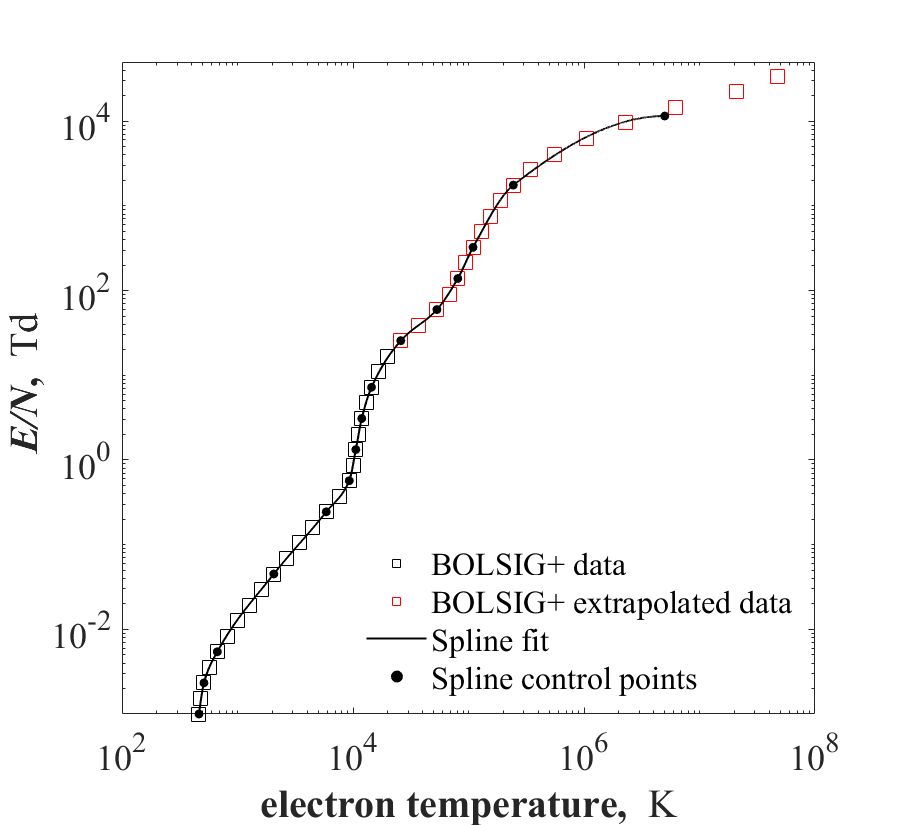
\includegraphics[width=0.99\linewidth, angle=0.0,scale=0.49]{electronimpact_figs/electronimpact_figure5.png}}
\subfigure[]{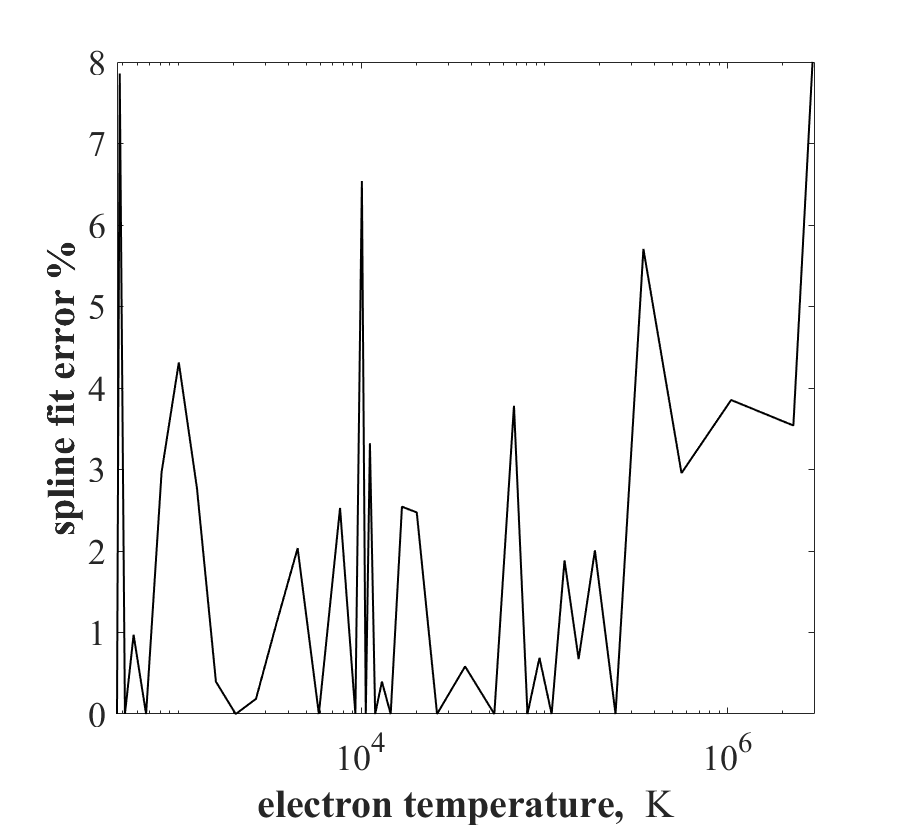
\includegraphics[width=0.99\linewidth, angle=0.0,scale=0.49]{electronimpact_figs/electronimpact_figure5_error.png}}
\caption{$E/N$ results for $\rm O$, showing (a) reduced electric field as a function of the electron temperature and (b) error percentage when fitting a cubic spline through BOLSIG+ data. The electron impact cross-sectional data used in the BOLSIG+ calculation is sourced from the Morgan database, Ref.\ \cite{lxc:2024:morgan}.}
\label{fig:electronimpact_5}
\end{figure}
%

\subsection{Nitrogen molecule ($\rm N_2$)}

Experimental data for $E/N$ vs electron temperature is available from Ch.\ 21 of Ref.\ \citen{book:1997:grigoriev} for $\rm N_2$. In this case a cubic spline is fitted through the experimental data points and also through the remaining lower and upper ranges, if any, for which there is BOLSIG+ data. All the processes involving cross-sections used in the BOLSIG+ calculation are given in Table \ref{tab:tableN2}. The reduced electric field results are shown in Fig. \ref{fig:electronimpact_1}. 

\begin{table*}[!htbp]
  \center\fontsizetable
  \begin{threeparttable}
    \tablecaption{$\rm N_2$ electron impact processes with available cross-section data.}
    \label{tab:tableN2}
    \fontsizetable
    \begin{tabular*}{\textwidth}{l@{\extracolsep{\fill}}llll}
    \toprule
    {no.}  & {process} & {type} &  {eV range}  &  {ref.} \\
    \midrule
      1 & $\rm e^- + N_2 \rightarrow N_2^+ + e^- + e^-$  &  ionization    &  15.6-1500 &   \cite{lxc:2024:morgan} \\ 
      \midrule     
      2 & $\rm e^- + N_2 \rightarrow e^- + N_2$  &  momentum transfer   &  0-1000  & \cite{lxc:2024:morgan}\\   
      \midrule
      3 & $\rm e^- + N_2 \rightarrow e^- + N_2^* $  &  rotational excitation   &  0.02-35 & \cite{lxc:2024:morgan}\\ 
           \midrule
      4 & $\rm e^- + N_2 \rightarrow e^- + N_2$$(\nu_1)$  &  vibrational excitation   &  0.290-35 &\cite{lxc:2024:morgan}\\  
      5 & $\rm e^- + N_2 \rightarrow e^- + N_2$$(\nu_1)$  &  vibrational excitation   &  0.291-35 &\cite{lxc:2024:morgan}\\  
      6 & $\rm e^- + N_2 \rightarrow e^- + N_2$$(\nu_2)$  &  vibrational excitation   &  0.590-35 &\cite{lxc:2024:morgan}\\ 
      7 & $\rm e^- + N_2 \rightarrow e^- + N_2$$(\nu_3)$  &  vibrational excitation   &  0.880-35 &\cite{lxc:2024:morgan}\\ 
      8 & $\rm e^- + N_2 \rightarrow e^- + N_2$$(\nu_4)$  &  vibrational excitation   &  1.170-35 &\cite{lxc:2024:morgan}\\ 
      9 & $\rm e^- + N_2 \rightarrow e^- + N_2$$(\nu_5)$  &  vibrational excitation   &  1.470-35 &\cite{lxc:2024:morgan}\\
      10 & $\rm e^- + N_2 \rightarrow e^- + N_2$$(\nu_6)$  &  vibrational excitation   &  1.760-35 &\cite{lxc:2024:morgan}\\ 
      11 & $\rm e^- + N_2 \rightarrow e^- + N_2$$(\nu_7)$  &  vibrational excitation   &  2.060-35 &\cite{lxc:2024:morgan}\\ 
      12 & $\rm e^- + N_2 \rightarrow e^- + N_2$$(\nu_8)$  &  vibrational excitation   &  2.350-35 &\cite{lxc:2024:morgan}\\ 
          \midrule
      13 & $\rm e^- + N_2 \rightarrow e^- + N_2$$(A^3 \Sigma_{u}^+) $  &  electronic excitation   &  6.170-35 & \cite{lxc:2024:morgan}\\ 
      14 & $\rm e^- + N_2 \rightarrow e^- + N_2$$(A^3 \Sigma_{u}^+)$  &  electronic excitation   &  7.000-35 & \cite{lxc:2024:morgan}\\ 
      15 & $\rm e^- + N_2 \rightarrow e^- + N_2$$(B^3 \Pi_{g}) $  &  electronic excitation   &  7.350-35 & \cite{lxc:2024:morgan}\\ 
      16 & $\rm e^- + N_2 \rightarrow e^- + N_2$$(W^3 \Delta) $  &  electronic excitation   &  7.360-35 & \cite{lxc:2024:morgan}\\ 
      17 & $\rm e^- + N_2 \rightarrow e^- + N_2$$(A^3 \Sigma_{u}^+) $  &  electronic excitation   &  7.80-35 & \cite{lxc:2024:morgan}\\ 
      18 & $\rm e^- + N_2 \rightarrow e^- + N_2$$(B^3 \Sigma) $  &  electronic excitation   &  8.16-35 & \cite{lxc:2024:morgan}\\ 
      19 & $\rm e^- + N_2 \rightarrow e^- + N_2$$(A^1 \Sigma) $  &  electronic excitation   &  8.40-35 & \cite{lxc:2024:morgan}\\ 
      20 & $\rm e^- + N_2 \rightarrow e^- + N_2$$(A^1 \Pi) $  &  electronic excitation   &  8.55-35 & \cite{lxc:2024:morgan}\\ 
      21 & $\rm e^- + N_2 \rightarrow e^- + N_2$$(W^1 \Delta) $  &  electronic excitation   &  8.89-35 & \cite{lxc:2024:morgan}\\ 
      22 & $\rm e^- + N_2 \rightarrow e^- + N_2$$(C^3 \Pi) $  &  electronic excitation   &  11.03-35 & \cite{lxc:2024:morgan}\\ 
      23 & $\rm e^- + N_2 \rightarrow e^- + N_2$$(E^3 \Sigma) $  &  electronic excitation   &  11.88-35 & \cite{lxc:2024:morgan}\\  
      24 & $\rm e^- + N_2 \rightarrow e^- + N_2$$(A^1 \Sigma) $  &  electronic excitation   &  12.25-35 & \cite{lxc:2024:morgan}\\ 
      25 & $\rm e^- + N_2 \rightarrow e^- + N + N $  &  electronic excitation   &  13.00-35 & \cite{lxc:2024:morgan}\\ 
    \bottomrule
    \end{tabular*}
   \end{threeparttable}
\end{table*}

\begin{figure}[!htbp]
\subfigure[]{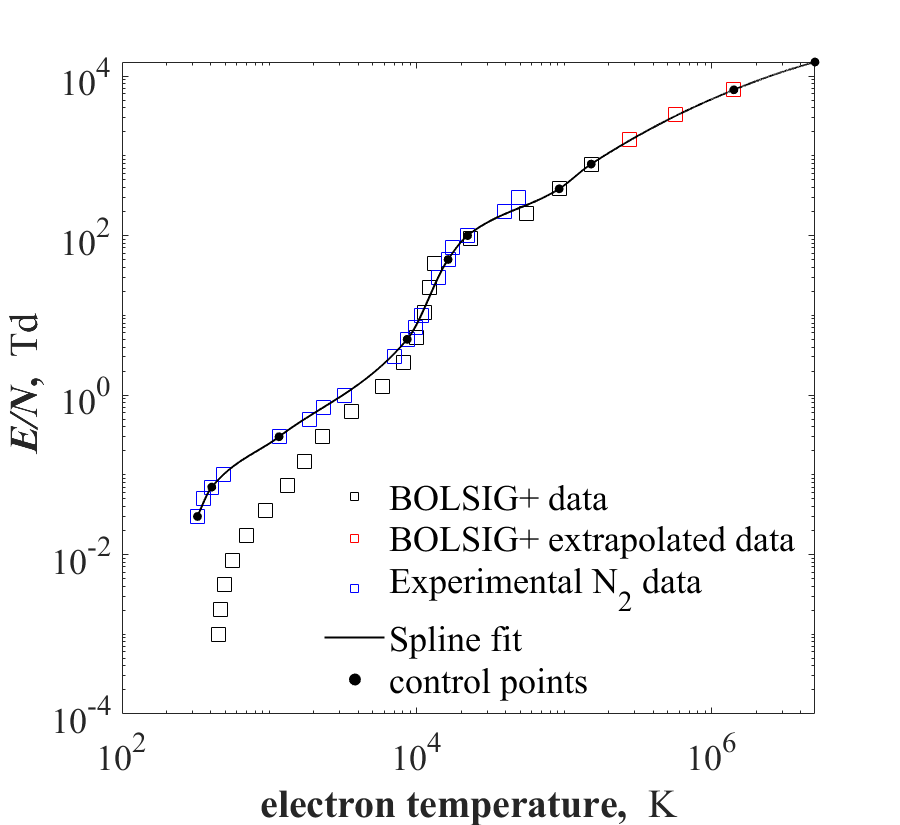
\includegraphics[width=0.99\linewidth, angle=0.0,scale=0.49]{electronimpact_figs/electronimpact_figure1.png}}
\subfigure[]{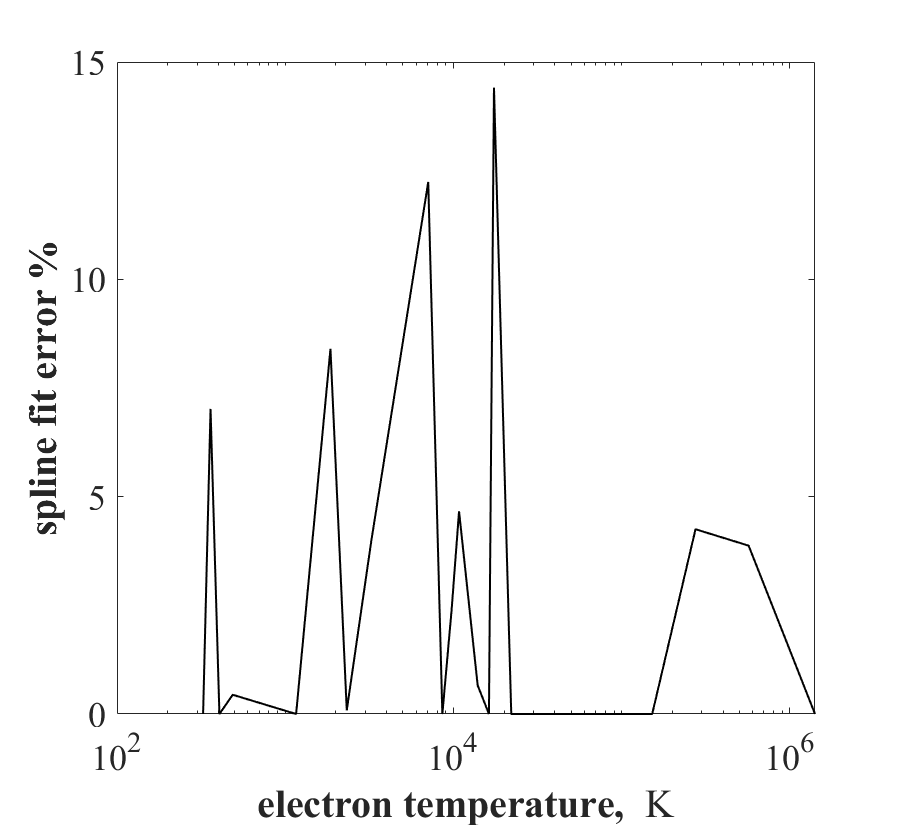
\includegraphics[width=0.99\linewidth, angle=0.0,scale=0.49]{electronimpact_figs/electronimpact_figure1_error.png}}
\caption{$E/N$ results for $\rm N_2$, showing (a) reduced electric field as a function of the electron temperature and (b) error percentage when fitting a cubic spline through the data. Experimental $\rm N_2$ data points are taken from Ref.\ \citen{book:1997:grigoriev}.}
\label{fig:electronimpact_1}
\end{figure}
%
\subsection{Oxygen molecule ($\rm O_2$)}

All the processes involving cross-sections used in the BOLSIG+ calculation are given in Table \ref{tab:tableO2}. Experimental data for $E/N$ vs electron temperature is available from Ch.\ 21 of Ref.\ \citen{book:1997:grigoriev} for $\rm O_2$. A cubic spline is fitted through the experimental data points and also through the remaining lower and upper ranges, if any, for which there is BOLSIG+ data.  The reduced electric field results are shown in Fig. \ref{fig:electronimpact_2}. In this case, no experimental data is available for $T_{\rm e}<1000$ K. Rather than make use of the BOLSIG+ results at low electron temperature which might not be accurate, we here prefer to extrapolate from the experimental data to lower $T_{\rm e}$. To do this, the experimental results for air are used and the corresponding $E/N$ value is obtained by summing the $\rm N_2$, $\rm O_2$ $E/N$ results weighed by their corresponding composition in dry air. The extrapolation of the $\rm O_2$ curve for $T_{\rm e}<1000$ K is such that there is good agreement between the experimental data and spline curve fit for air. The latter is shown in Fig. \ref{fig:electronimpact_2}. All the processes involving cross-sections used in the BOLSIG+ calculation are given in Table \ref{tab:tableO2}.
%



\begin{table*}[!htbp]
  \center\fontsizetable
  \begin{threeparttable}
    \tablecaption{$\rm O_2$ electron impact processes with available cross-section data.}
    \label{tab:tableO2}
    \fontsizetable
    \begin{tabular*}{\textwidth}{l@{\extracolsep{\fill}}llll}
    \toprule
    {no.}  & {process} & {type} &  {eV range}  &  {ref.} \\
    \midrule
      1 & $\rm e^- + O_2 \rightarrow O_2^+ + e^- + e^-$  &  ionization   &  12.6-1500 &   \cite{lxc:2024:morgan} \\ 
      \midrule     
      2 & $\rm e^- + O_2 \rightarrow e^- + O_2$  &  momentum transfer   &  0-1000  & \cite{lxc:2024:morgan}\\   
      \midrule
      3 & $\rm e^- + O_2 \rightarrow e^- + O_2^* $  &  rotational excitation   &  0.38-20 & \cite{lxc:2024:morgan}\\ 
           \midrule
      4 & $\rm e^- + O_2 \rightarrow e^- + O_2$$(\nu_1) $  &  vibrational excitation   &  0.57-15 &\cite{lxc:2024:morgan}\\  
      5 & $\rm e^- + O_2 \rightarrow e^- + O_2$$(\nu_2) $  &  vibrational excitation   &  0.75-15 &\cite{lxc:2024:morgan}\\ 
          \midrule
      6 & $\rm e^- + O_2 \rightarrow e^- + O_2$$(A^1 \Delta) $  &  electronic excitation   &  0.977-45 & \cite{lxc:2024:morgan}\\ 
      7 & $\rm e^- + O_2 \rightarrow e^- + O_2$$(B^1 \Sigma) $  &  electronic excitation   &  1.627-45 & \cite{lxc:2024:morgan}\\ 
      8 & $\rm e^- + O_2 \rightarrow e^- + O_2(-) $  &  electronic excitation   &  4.50-45 & \cite{lxc:2024:morgan}\\ 
      9 & $\rm e^- + O_2 \rightarrow e^- + O_2(-) $  &  electronic excitation   &  6.00-45 & \cite{lxc:2024:morgan}\\ 
      10 & $\rm e^- + O_2 \rightarrow e^- + O_2(-) $  &  electronic excitation   &  8.40-45 & \cite{lxc:2024:morgan}\\ 
      11 & $\rm e^- + O_2 \rightarrow e^- + O_2(-) $  &  electronic excitation   &  9.97-100 & \cite{lxc:2024:morgan}\\ 
      12 & $\rm e^- + O_2 \rightarrow e^- + O + O $  &  electronic excitation   &  14.70-100 & \cite{lxc:2024:morgan}\\ 
    \bottomrule
    \end{tabular*}

   \end{threeparttable}
\end{table*}
%
\begin{figure}[!htbp]
\subfigure[]{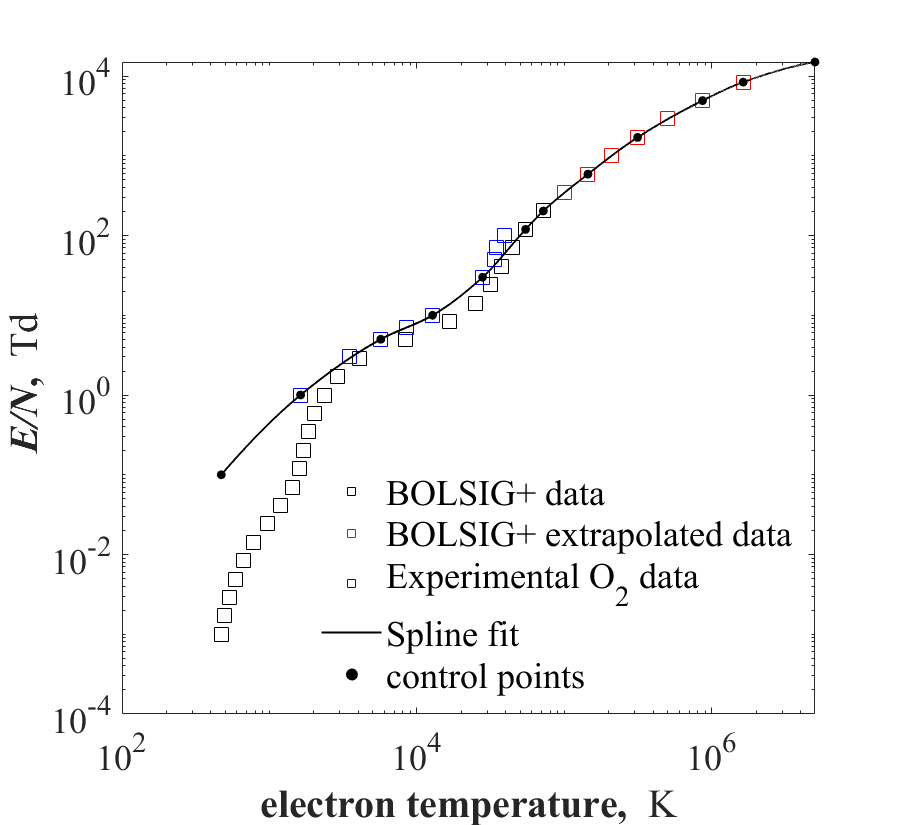
\includegraphics[width=0.99\linewidth, angle=0.0,scale=0.49]{electronimpact_figs/electronimpact_figure2.png}}
\subfigure[]{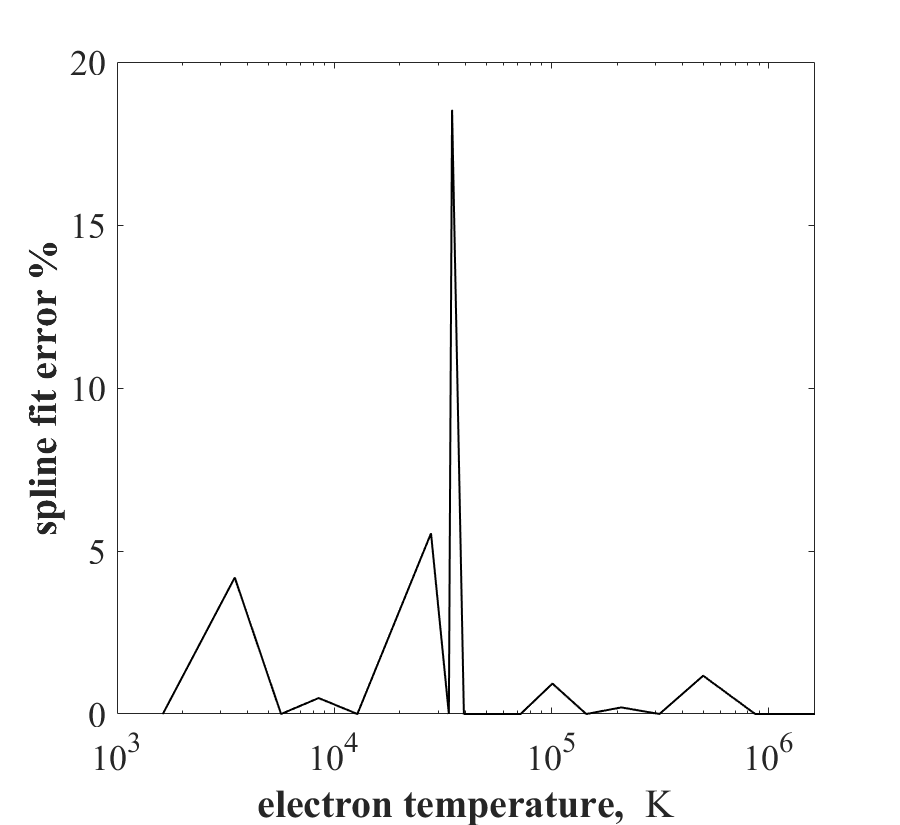
\includegraphics[width=0.99\linewidth, angle=0.0,scale=0.49]{electronimpact_figs/electronimpact_figure2_error.png}}
\caption{$E/N$ results for $\rm O_2$, showing (a) reduced electric field as a function of the electron temperature and (b) error percentage when fitting a cubic spline through the data. Experimental $\rm O_2$ data points are taken from \citen{book:1997:grigoriev}.}
\label{fig:electronimpact_2}
\end{figure}


%
\subsection{Nitric oxide ($\rm NO$)}

The results for NO are obtained by fitting a spline through BOLSIG+ and known experimental data. For electron temperatures less than 1000 K, the reduced electric field is computed assuming that the corresponding electron energy loss function $\zeta_{\rm e} $ in the local approximation takes the floor value of 0.001 according to the following equation:
%
\begin{equation}
\zeta_{\rm e}   =    \frac{2 m_{\rm e} \mu_{\rm e} N}{3  k_{\rm B} T_{\rm e} } \left[  \mu_{\rm e}N  \left(E/N(T_{\rm e})\right)^2\right]
\end{equation}
%
The final curve fit is shown in Fig. \ref{fig:electronimpact_3} alongside all the reference data used to obtain it. All the processes involving cross-sections used in the BOLSIG+ calculation are given in Table \ref{tab:tableNO}.

\begin{table*}[!htbp]
  \center\fontsizetable
  \begin{threeparttable}
    \tablecaption{$\rm NO$ electron impact processes with available cross-section data.}
    \label{tab:tableNO}
    \fontsizetable
    \begin{tabular*}{\textwidth}{l@{\extracolsep{\fill}}llll}
    \toprule
    {no.}  & {process} & {type} &  {eV range}  &  {ref.} \\
    \midrule
      1 & $\rm e^- + NO \rightarrow NO^+ + e^- + e^-$  &  ionization   &  9.26-1000 &   \cite{lxc:2024:morgan} \\ 
      \midrule     
      2 & $\rm e^- + NO \rightarrow e^- + NO$  &  momentum transfer   &  0.0-100  & \cite{lxc:2024:morgan}\\   
      \midrule
      3 & $\rm e^- + NO \rightarrow e^- + NO$$(\nu_1) $  &  vibrational excitation   &  0.30-100 & \cite{lxc:2024:morgan}\\ 
      4 & $\rm e^- + NO \rightarrow e^- + NO$$(\nu_2) $  &  vibrational excitation   &  0.45-100 & \cite{lxc:2024:morgan}\\ 
      5 & $\rm e^- + NO \rightarrow e^- + NO$$(\nu_3) $  &  vibrational excitation   &  0.75-100 & \cite{lxc:2024:morgan}\\ 
      6 & $\rm e^- + NO \rightarrow e^- + NO$$(\nu_4) $  &  vibrational excitation   &  0.90-100 & \cite{lxc:2024:morgan}\\ 
      7 & $\rm e^- + NO \rightarrow e^- + NO$$(\nu_5) $  &  vibrational excitation   &  1.20-100 & \cite{lxc:2024:morgan}\\ 
      8 & $\rm e^- + NO \rightarrow e^- + NO$$(\nu_6) $  &  vibrational excitation   &  1.35-100 & \cite{lxc:2024:morgan}\\ 
     \midrule
      9 & $\rm e^- + NO \rightarrow e^- + NO^* $  &  electronic excitation   &  5.50-100 & \cite{lxc:2024:morgan}\\ 
     10 & $\rm e^- + NO \rightarrow e^- + NO^* $  &  electronic excitation   &  6.60-100 & \cite{lxc:2024:morgan}\\
     11 & $\rm e^- + NO \rightarrow e^- + NO^* $  &  electronic excitation   &  9.26-100 & \cite{lxc:2024:morgan}\\
    \bottomrule
    \end{tabular*}
   \end{threeparttable}
\end{table*}

\begin{figure}[!htbp]
\subfigure[]{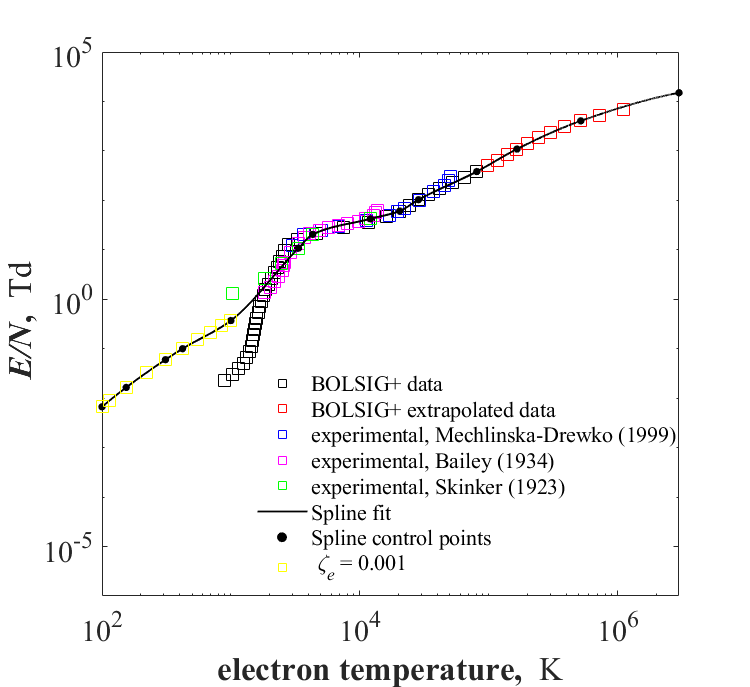
\includegraphics[width=0.99\linewidth, angle=0.0,scale=0.49]{electronimpact_figs/electronimpact_figure3.png}}
\subfigure[]{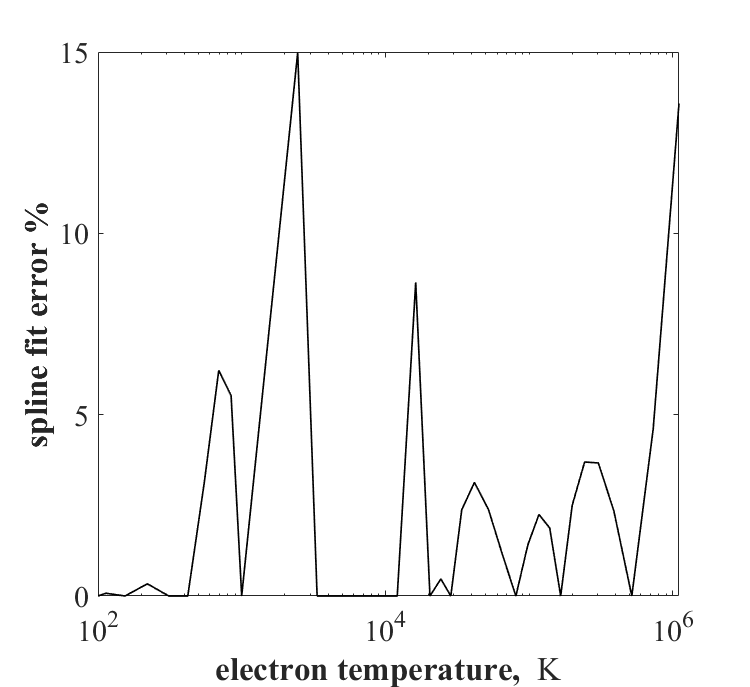
\includegraphics[width=0.99\linewidth, angle=0.0,scale=0.49]{electronimpact_figs/electronimpact_figure3_error.png}}
\caption{$E/N$ results for $\rm NO$, showing (a) reduced electric field as a function of the electron temperature and (b) error percentage when fitting a cubic spline through the data. Experimental data points are taken from Fig.\ 2 of Ref.\ \citen{jop:1999:mechlinska}, Fig.\ 5 of Ref.\ \citen{jos:1934:bailey} and Fig.\ 1.32 of Ref.\ \citen{jos:1934:skinker}. For electron temperatures less than 1000 K, the $E/N$ values are estimated by assuming a value of electron energy loss function $\zeta_{\rm e} = 0.001$. }
\label{fig:electronimpact_3}
\end{figure}
%
All the processes involving cross-sections used in the BOLSIG+ calculation are given in Table \ref{tab:tableNH3}. The reduced electric field results are shown in Fig. \ref{fig:electronimpact_3}.
%
\subsection{Ammonia ($\rm NH_3$)}

All the processes involving cross-sections used in the BOLSIG+ calculation are given in Table \ref{tab:tableNH3}. The reduced electric field results are shown in Fig. \ref{fig:electronimpact_6}.

\begin{table*}[!htbp]
  \center\fontsizetable
  \begin{threeparttable}
    \tablecaption{$\rm NH_3$ electron impact processes with available cross-section data.}
    \label{tab:tableNH3}
    \fontsizetable
    \begin{tabular*}{\textwidth}{l@{\extracolsep{\fill}}llll}
    \toprule
    {no.}  & {process} & {type} &  {eV range}  &  {ref.} \\
    \midrule
      1 & $\rm e^- + NH_3 \rightarrow NH + H_2^+ + e^- + e^-$  &  ionization   &  10-1000 &  \cite{psst:2023:snoeckx} \\
      2 & $\rm e^- + NH_3 \rightarrow NH_3^+ + e^- + e^-$  &  ionization   &  10-1000  & \cite{psst:2023:snoeckx}\\
      3 & $\rm e^- + NH_3 \rightarrow NH_2 + H^+ + e^- + e^-$  &  ionization   &  20-1000   &\cite{psst:2023:snoeckx}\\
      4 & $\rm e^- + NH_3 \rightarrow NH_2^+ + H + e^- + e^-$  &  ionization   &  10-1000  & \cite{psst:2023:snoeckx}\\      
      5 & $\rm e^- + NH_3 \rightarrow N^+ + H_2 + H + e^- + e^-$  &  ionization   &  10-1000   &\cite{psst:2023:snoeckx}\\         
      6 & $\rm e^- + NH_3 \rightarrow NH^+ + H_2 +  e^- + e^-$  &  ionization   &  20-1000   &\cite{psst:2023:snoeckx}\\  
      \midrule     
      7 & $\rm e^- + NH_3 \rightarrow e^- + NH_3$  &  momentum transfer   &  0-4000  & \cite{lxc:2024:morgan}\\   
      \midrule
      8 & $\rm e^- + NH_3 \rightarrow e^- + NH_3(V2)$  &  electronic excitation   &  0.118-1000 & \cite{lxc:2024:morgan}\\ 
      9 & $\rm e^- + NH_3 \rightarrow e^- + NH_3(V4)$  &  electronic excitation   &  0.202-1000 &\cite{lxc:2024:morgan}\\  
      10 & $\rm e^- + NH_3 \rightarrow e^- + NH_3(V13)$  &  electronic excitation   &  0.420-1000 &\cite{lxc:2024:morgan}\\  
      11 & $\rm e^- + NH_3 \rightarrow e^- + NH_3(E1)$  &  electronic excitation   &  5.720-1000 &\cite{lxc:2024:morgan}\\ 
      12 & $\rm e^- + NH_3 \rightarrow e^- + NH_3(E2)$  &  electronic excitation   &  8.650-1000 &\cite{lxc:2024:morgan}\\ 
      \midrule
      13 & $\rm e^- + NH_3 \rightarrow e^- + NH_3(\nu_1)$  &  vibrational excitation   &  0.42-34 &\cite{psst:2023:snoeckx}\\  
      14 & $\rm e^- + NH_3 \rightarrow e^- + NH_3(\nu_2)$  &  vibrational excitation   &  0.12-32 &\cite{psst:2023:snoeckx}\\ 
      15 & $\rm e^- + NH_3 \rightarrow e^- + NH_3(\nu_3)$  &  vibrational excitation   &  0.45-35 &\cite{psst:2023:snoeckx}\\ 
      16 & $\rm e^- + NH_3 \rightarrow e^- + NH_3(\nu_4)$  &  vibrational excitation   &  0.21-35 &\cite{psst:2023:snoeckx}\\ 
      \midrule
      17 & $\rm e^- + NH_3 \rightarrow e^- + NH_3(00\rightarrow10)$  &  rotational excitation   &  0.01-30 & \cite{psst:2023:snoeckx}\\ 
      18 & $\rm e^- + NH_3 \rightarrow e^- + NH_3(00\rightarrow20)$  &  rotational excitation   &  0.01-30 &\cite{psst:2023:snoeckx}\\ 
      19 & $\rm e^- + NH_3 \rightarrow e^- + NH_3(00\rightarrow30)$  &  rotational excitation   &  0.01-30 &\cite{psst:2023:snoeckx}\\ 
      20 & $\rm e^- + NH_3 \rightarrow e^- + NH_3(00\rightarrow40)$  &  rotational excitation   &  0.01-30 &\cite{psst:2023:snoeckx}\\ 
      21 & $\rm e^- + NH_3 \rightarrow e^- + NH_3(00\rightarrow50)$  &  rotational excitation   &  0.01-30 &\cite{psst:2023:snoeckx}\\ 
    \bottomrule
    \end{tabular*}
   \end{threeparttable}
\end{table*}
%
\begin{figure}[!htbp]
\subfigure[]{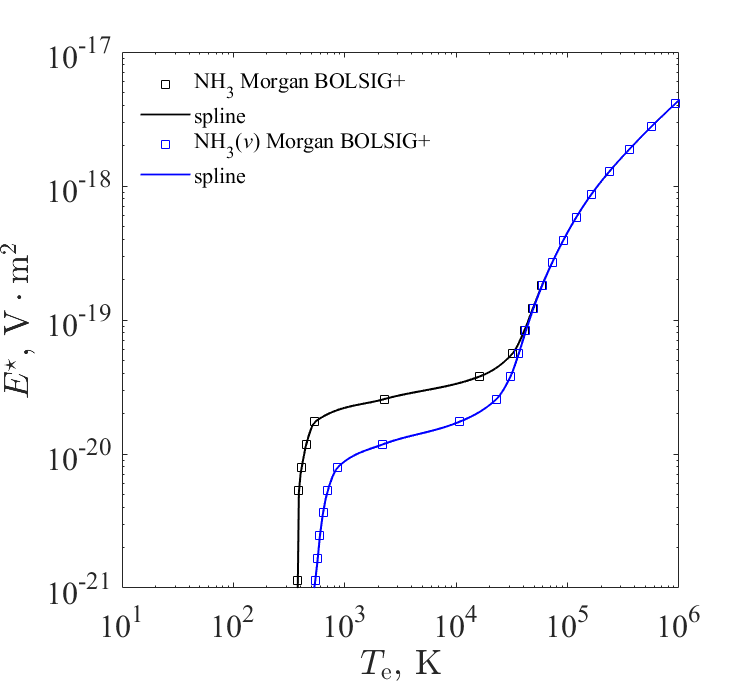
\includegraphics[width=0.99\linewidth, angle=0.0,scale=0.49]{electronimpact_figs/electronimpact_figure6.png}}
\subfigure[]{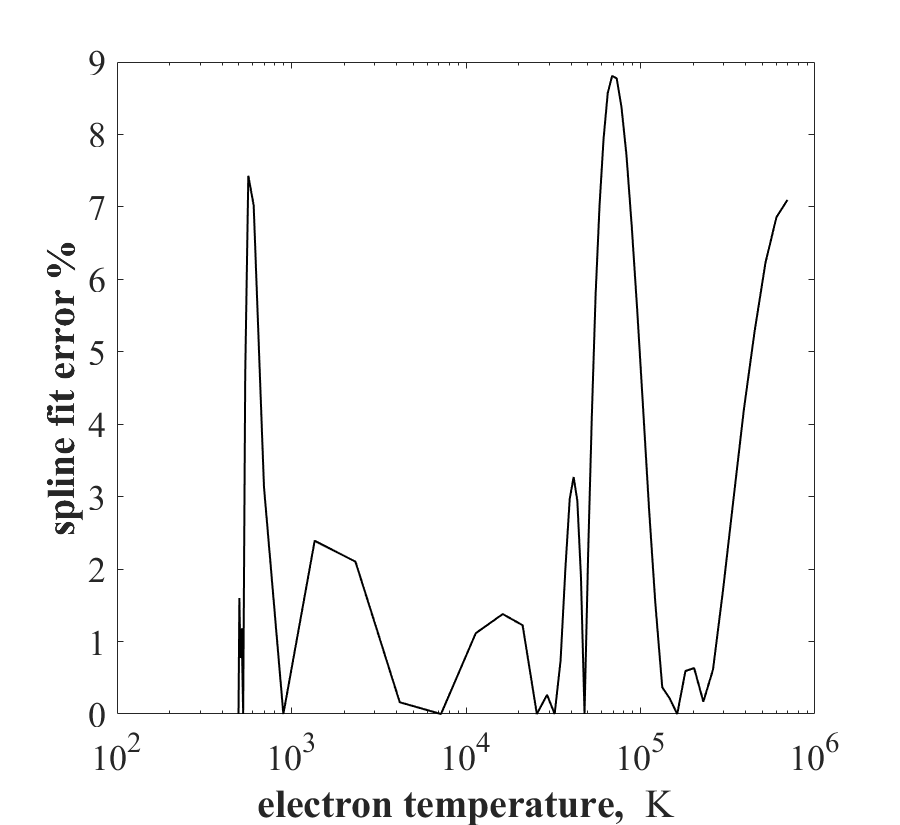
\includegraphics[width=0.99\linewidth, angle=0.0,scale=0.49]{electronimpact_figs/electronimpact_figure6_error.png}}
\caption{$E/N$ results for $\rm NH_3$, showing (a) reduced electric field as a function of the electron temperature and (b) error percentage when fitting a cubic spline through the data. The electron impact cross-sectional data used in the BOLSIG+ calculation is sourced from the Hayashi database, Ref.\ \cite{springer:1987:hayashi}.}
\label{fig:electronimpact_6}
\end{figure}
%
\subsection{Ammonia (vibrationally excited state $\rm NH_3$$(v)$)}

The reduced electric field results are shown in Fig. \ref{fig:electronimpact_NH3v}. The cross-sections for electron impact with this vibrationally excited state of ammonia are obtained by shifting the energy threshold of all electron impact processes by +0.118 eV from the cross-section data of ground state ammonia.
%
\begin{figure}[!htbp]
\subfigure[]{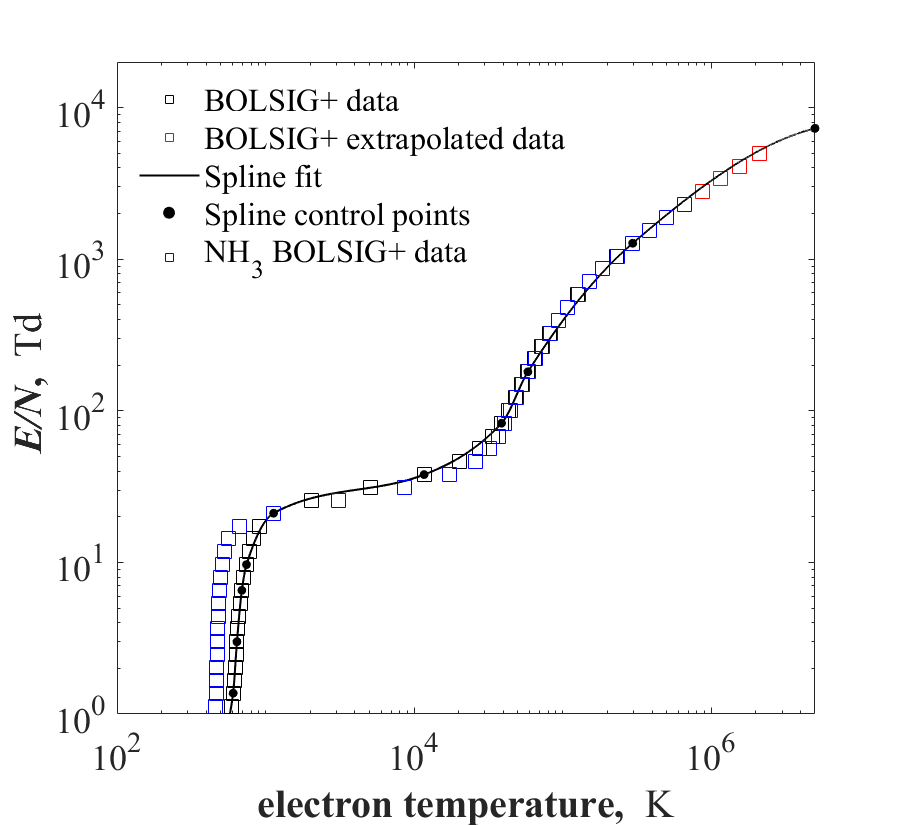
\includegraphics[width=0.99\linewidth, angle=0.0,scale=0.49]{electronimpact_figs/electronimpact_figureNH3v.png}}
\subfigure[]{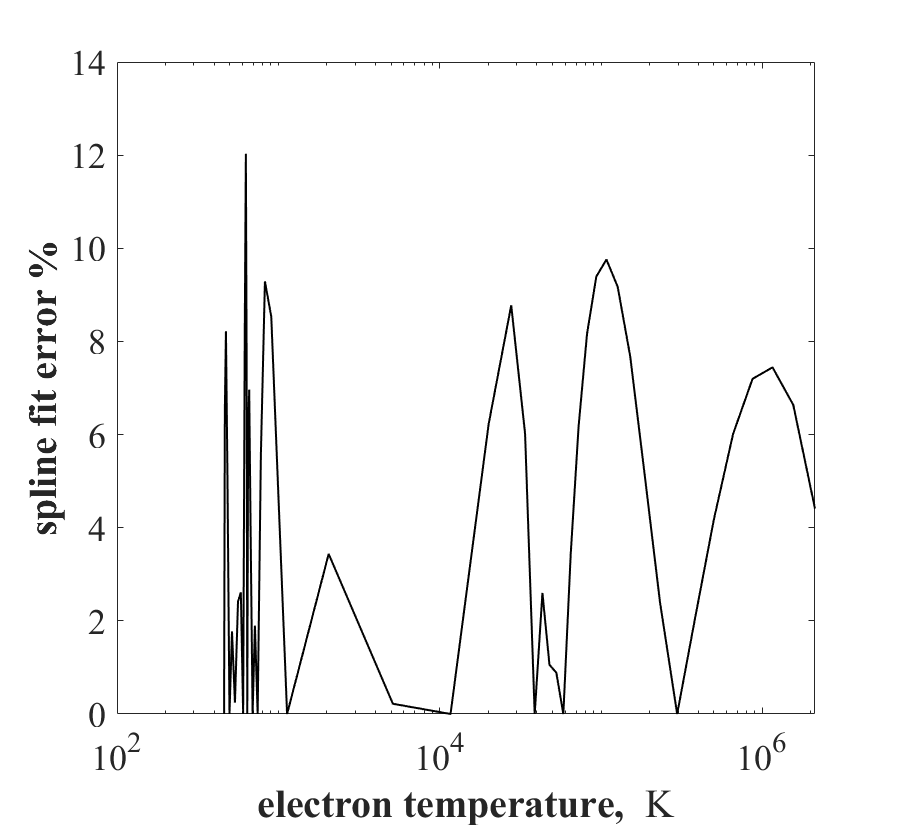
\includegraphics[width=0.99\linewidth, angle=0.0,scale=0.49]{electronimpact_figs/electronimpact_figureNH3v_error.png}}
\caption{$E/N$ results for $\rm NH_3$$(v)$, showing (a) reduced electric field as a function of the electron temperature and (b) error percentage when fitting a cubic spline through the data. The electron impact cross-sectional data used in the BOLSIG+ calculation is sourced from the Hayashi database, Ref.\ \cite{springer:1987:hayashi}.}
\label{fig:electronimpact_NH3v}
\end{figure}
%


\subsection{Ethylene ($\rm C_2H_4$)}

The reduced electric field results are shown in Fig. \ref{fig:electronimpact_C2H4}. The results for $\rm C_2H_4$ are obtained by fitting a spline through BOLSIG+ and known experimental data.

\begin{table*}[!htbp]
  \center\fontsizetable
  \begin{threeparttable}
    \tablecaption{$\rm C_2H_4$ electron impact processes with available cross-section data.}
    \label{tab:tableC2H4}
    \fontsizetable
    \begin{tabular*}{\textwidth}{l@{\extracolsep{\fill}}llll}
    \toprule
    {no.}  & {process} & {type} &  {eV range}  &  {ref.} \\
    \midrule
      1 & $\rm e^- + C_2H_4 \rightarrow C_2H_4^+ + e^- + e^-$  &  ionization   &  10.507-930 &   \cite{lxc:2024:morgan} \\ 
      \midrule     
      2 & $\rm e^- + C_2H_4 \rightarrow e^- + C_2H_4$  &  momentum transfer   &  0.0-878  & \cite{lxc:2024:morgan}\\   
      \midrule
      3 & $\rm e^- + C_2H_4 \rightarrow e^- + C_2H_4^*$  &   excitation   &  0.11-260 & \cite{lxc:2024:morgan}\\ 
      4 & $\rm e^- + C_2H_4 \rightarrow e^- + C_2H_4^*$  &   excitation   &  0.36-74 & \cite{lxc:2024:morgan}\\ 
      5 & $\rm e^- + C_2H_4 \rightarrow e^- + C_2H_4^*$  &   excitation   &  3.8-30.5 & \cite{lxc:2024:morgan}\\ 
      6 & $\rm e^- + C_2H_4 \rightarrow e^- + C_2H_4^*$  &   excitation   &  5.0-925 & \cite{lxc:2024:morgan}\\ 
      7 & $\rm e^- + C_2H_4 \rightarrow e^- + C_2H_4^*$  &   excitation   &  7.0-918 & \cite{lxc:2024:morgan}\\ 
    \bottomrule
    \end{tabular*}
   \end{threeparttable}
\end{table*}

%
\begin{figure}[!htbp]
\centering
\subfigure[]{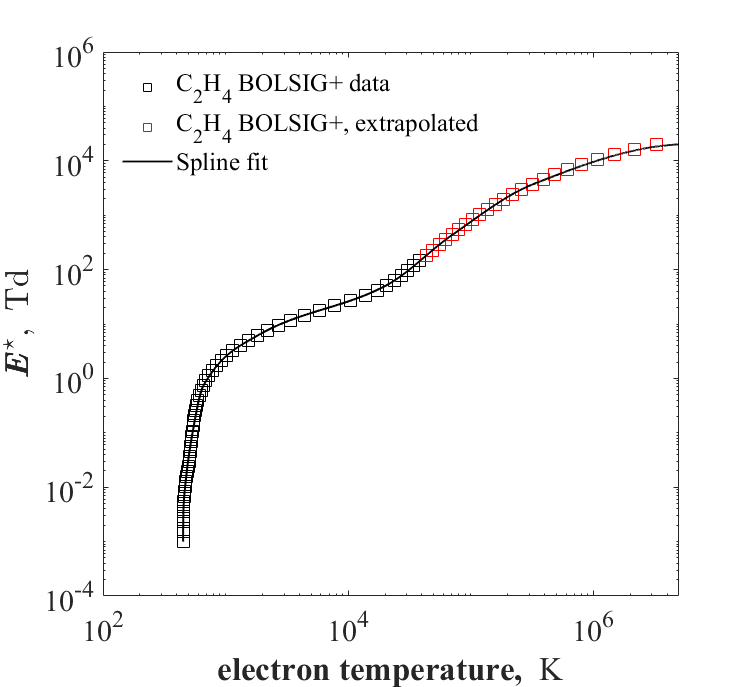
\includegraphics[width=0.99\linewidth, angle=0.0,scale=0.49]{electronimpact_figs/electronimpact_figureC2H4.png}}
\subfigure[]{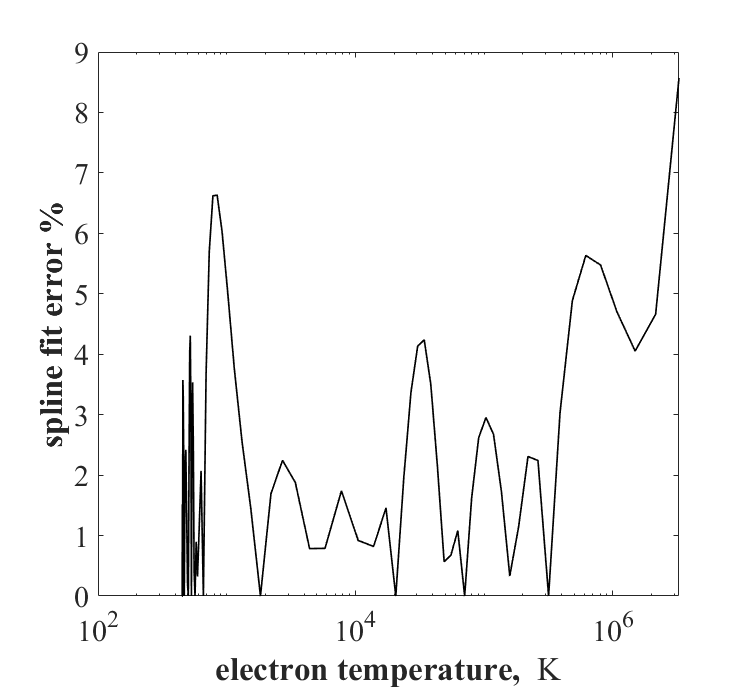
\includegraphics[width=0.99\linewidth, angle=0.0,scale=0.49]{electronimpact_figs/electronimpact_figureC2H4_error.png}}
\subfigure[]{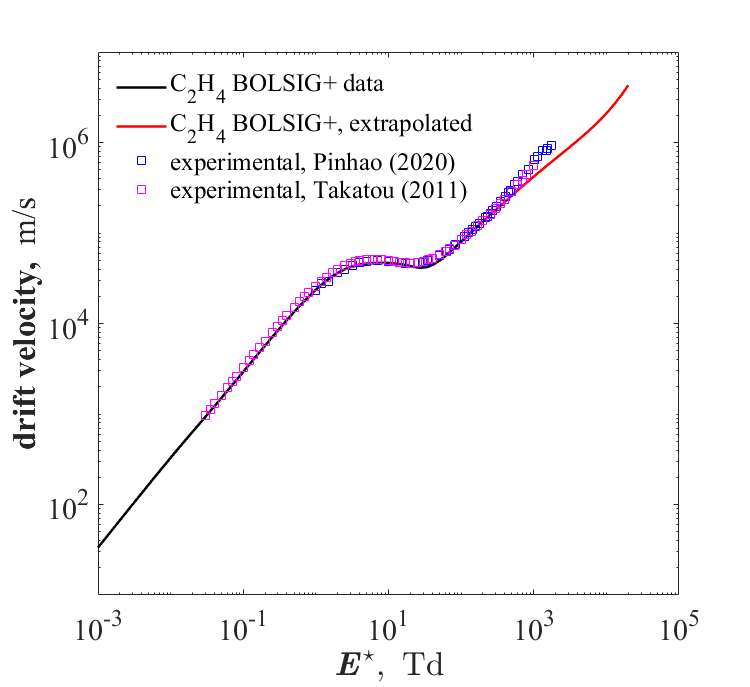
\includegraphics[width=0.99\linewidth, angle=0.0,scale=0.49]{electronimpact_figs/electronimpact_figureC2H4_drift.png}}
\caption{$E^\star$ results for $\rm C_2H_4$, showing (a) reduced electric field as a function of the electron temperature, b) error percentage when fitting a cubic spline through the data and (c) bulk drift velocity of electrons in ethylene as a function of the reduced electric field. The electron impact cross-sectional data used in the BOLSIG+ calculation is sourced from the Morgan database, Ref.\ \cite{lxc:2024:morgan}. Experimental data points are taken from Fig. 4 of Ref.\ \cite{jop:2011:takatou} and Fig. 5 of Ref.\ \cite{psst:2020:pinhao}.}
\label{fig:electronimpact_C2H4}
\end{figure}
%

\subsection{Water vapor ($\rm H_2O$)}

The reduced electric field results are shown in Fig. \ref{fig:electronimpact_H2O}. The results for $\rm H_2O$ are obtained by fitting a spline through BOLSIG+ and known experimental data.
%

\begin{table*}[!htbp]
  \center\fontsizetable
  \begin{threeparttable}
    \tablecaption{$\rm H_2O$ electron impact processes with available cross-section data.}
    \label{tab:tableH2O}
    \fontsizetable
    \begin{tabular*}{\textwidth}{l@{\extracolsep{\fill}}llll}
    \toprule
    {no.}  & {process} & {type} &  {eV range}  &  {ref.} \\
    \midrule
      1 & $\rm e^- + H_2O \rightarrow H_2O^+ + e^- + e^-$  &  ionization   &  12.61-960 &   \cite{phig:1987:yousfi} \\ 
      \midrule     
      2 & $\rm e^- + H_2O \rightarrow e^- + H_2O$  &  momentum transfer   &  0.0-500  & \cite{phig:1987:yousfi}\\   
      \midrule
      3 & $\rm e^- + H_2O \rightarrow e^- + H_2O(\rm ROT)$  &  rotational excitation   &  0.04-1000 & \cite{phig:1987:yousfi}\\ 
      4 & $\rm e^- + H_2O \rightarrow e^- + H_2O(010)$  &   excitation   &  0.20-1000 & \cite{phig:1987:yousfi}\\ 
      5 & $\rm e^- + H_2O \rightarrow e^- + H_2O(101)$  &   excitation   &  0.45-1000 & \cite{phig:1987:yousfi}\\ 
      6 & $\rm e^- + H_2O \rightarrow e^- + H +OH$  &   excitation   &  7.10-500 & \cite{phig:1987:yousfi}\\ 
    \bottomrule
    \end{tabular*}
   \end{threeparttable}
\end{table*}

%
\begin{figure}[!htbp]
\centering
\subfigure[]{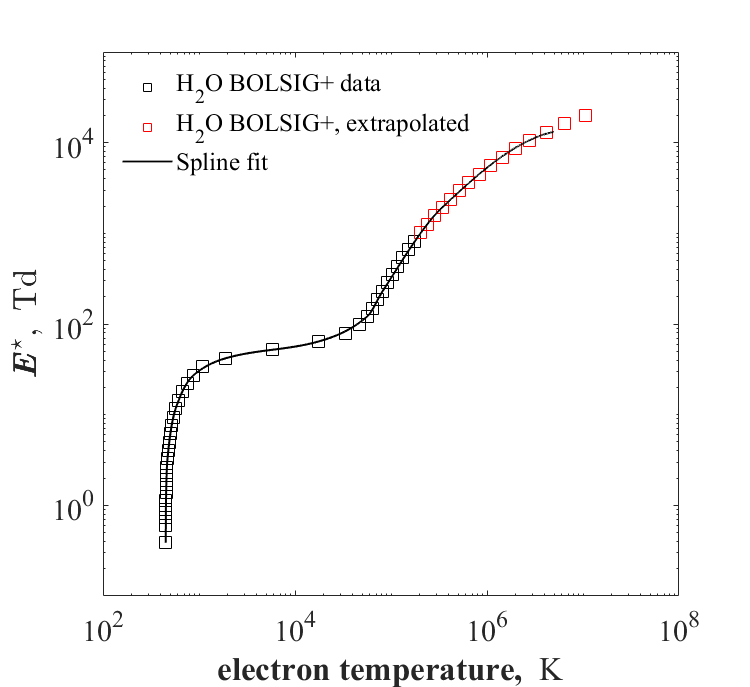
\includegraphics[width=0.99\linewidth, angle=0.0,scale=0.49]{electronimpact_figs/electronimpact_figureH2O.png}}
\subfigure[]{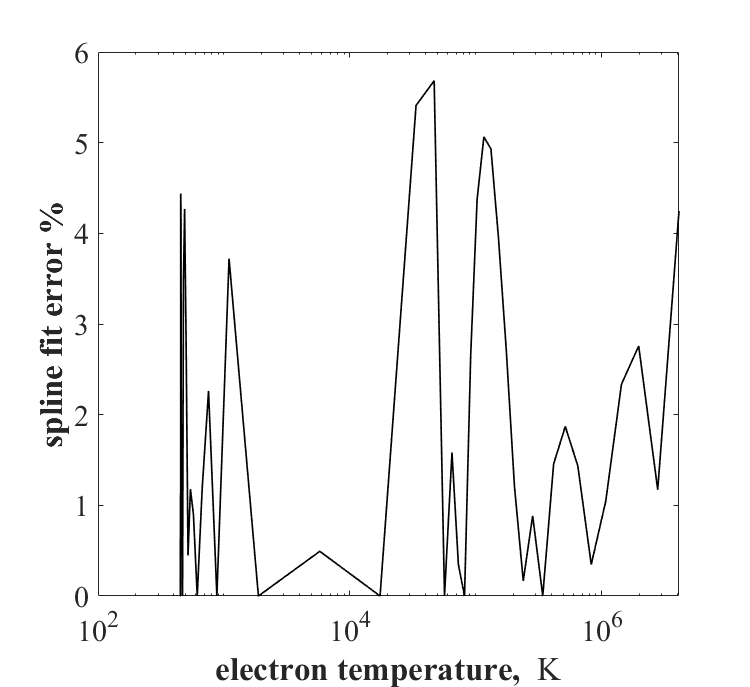
\includegraphics[width=0.99\linewidth, angle=0.0,scale=0.49]{electronimpact_figs/electronimpact_figureH2O_error.png}}
\subfigure[]{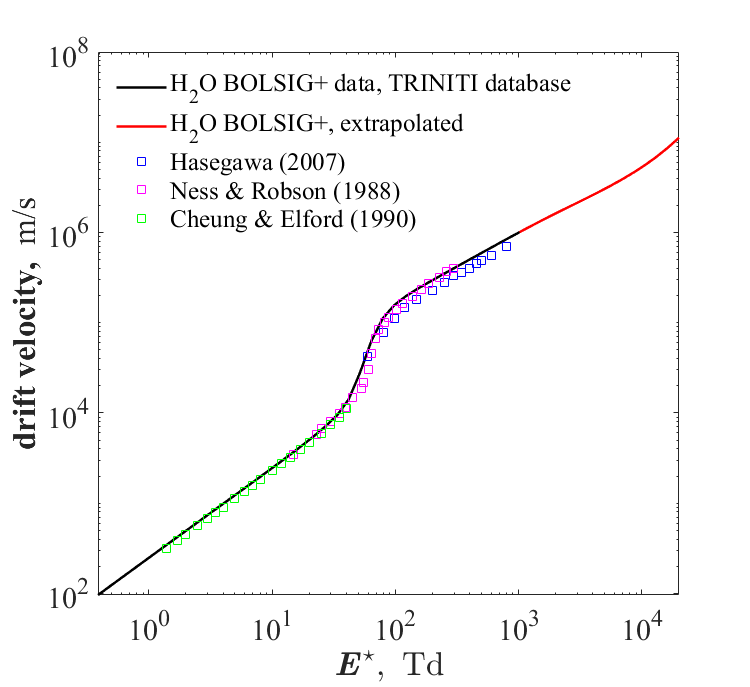
\includegraphics[width=0.99\linewidth, angle=0.0,scale=0.49]{electronimpact_figs/electronimpact_figureH2O_drift.png}}
\caption{$E^\star$ results for $\rm H_2O$, showing (a) reduced electric field as a function of the electron temperature, b) error percentage when fitting a cubic spline through the data and (c) bulk drift velocity of electrons in ethylene as a function of the reduced electric field. The electron impact cross-sectional data used in the BOLSIG+ calculation is sourced from the TRINITI lxcat database, Ref.\ \cite{phig:1987:yousfi}. Experimental data points are taken from Fig. 1. of Ref.\ \cite{jop:2007:hasegawa}, Fig. 4 of Ref.\ \cite{pra:1988:ness} and Table 1 of Ref.\ \cite{ajp:1990:cheung}.}
\label{fig:electronimpact_H2O}
\end{figure}
%

\subsection{Carbon monoxide ($\rm CO$)}

The reduced electric field results are shown in Fig. \ref{fig:electronimpact_CO}. The results for $\rm CO$ are obtained by fitting a spline through BOLSIG+ and known experimental data.

\begin{table*}[!htbp]
  \center\fontsizetable
  \begin{threeparttable}
    \tablecaption{$\rm CO$ electron impact processes with available cross-section data.}
    \label{tab:tableCO}
    \fontsizetable
    \begin{tabular*}{\textwidth}{l@{\extracolsep{\fill}}llll}
    \toprule
    {no.}  & {process} & {type} &  {eV range}  &  {ref.} \\
    \midrule
      1 & $\rm e^- + CO \rightarrow CO^+ + e^- + e^-$  &  ionization   &  14.01-100 &   \cite{lxc:2024:morgan} \\ 
      \midrule     
      2 & $\rm e^- + CO \rightarrow e^- + CO$  &  momentum transfer   &  0.0-1000 & \cite{lxc:2024:morgan}\\   
      \midrule
       3 & $\rm e^- + CO \rightarrow e^- + CO(V1)$  &   excitation   &  0.266-100 & \cite{lxc:2024:morgan}\\ 
      4 & $\rm e^- + CO \rightarrow e^- + CO(V2)$  &   excitation   &  0.528-100 & \cite{lxc:2024:morgan}\\ 
      5 & $\rm e^- + CO \rightarrow e^- + CO(V3)$  &   excitation   &  0.787-100 & \cite{lxc:2024:morgan}\\ 
      6 & $\rm e^- + CO \rightarrow e^- + CO(V4)$  &   excitation   &  1.04-100 & \cite{lxc:2024:morgan}\\ 
      7 & $\rm e^- + CO \rightarrow e^- + CO(V5)$  &   excitation   &  1.30-100 & \cite{lxc:2024:morgan}\\ 
      8 & $\rm e^- + CO \rightarrow e^- + CO(V6)$  &   excitation   &  1.54-100 & \cite{lxc:2024:morgan}\\ 
      9 & $\rm e^- + CO \rightarrow e^- + CO(V7)$  &   excitation   &  1.79-100 & \cite{lxc:2024:morgan}\\ 
      10 & $\rm e^- + CO \rightarrow e^- + CO(V8)$  &   excitation   &  2.03-100 & \cite{lxc:2024:morgan}\\ 
      11 & $\rm e^- + CO \rightarrow e^- + CO(V9)$  &   excitation   &  2.27-100 & \cite{lxc:2024:morgan}\\ 
      12 & $\rm e^- + CO \rightarrow e^- + CO(V10)$  &   excitation   &  2.51-100 & \cite{lxc:2024:morgan}\\ 
      13 & $\rm e^- + CO \rightarrow e^- + CO(A^3\Pi)$  &   electronic excitation   &  6.22-100 & \cite{lxc:2024:morgan}\\ 
      14 & $\rm e^- + CO \rightarrow e^- + CO(A^3\Sigma)$  &   electronic excitation   &  6.80-100 & \cite{lxc:2024:morgan}\\ 
      15 & $\rm e^- + CO \rightarrow e^- + CO(A^1\Pi)$  &   electronic excitation   &  7.90-100 & \cite{lxc:2024:morgan}\\ 
      16 & $\rm e^- + CO \rightarrow e^- + CO(B^3\Sigma)$  &   electronic excitation   &  10.4-100 & \cite{lxc:2024:morgan}\\ 
      17 & $\rm e^- + CO \rightarrow e^- + CO(C^1\Sigma)$  &   electronic excitation   &  10.6-100 & \cite{lxc:2024:morgan}\\ 
    \bottomrule
    \end{tabular*}
   \end{threeparttable}
\end{table*}

%
\begin{figure}[!htbp]
\centering
\subfigure[]{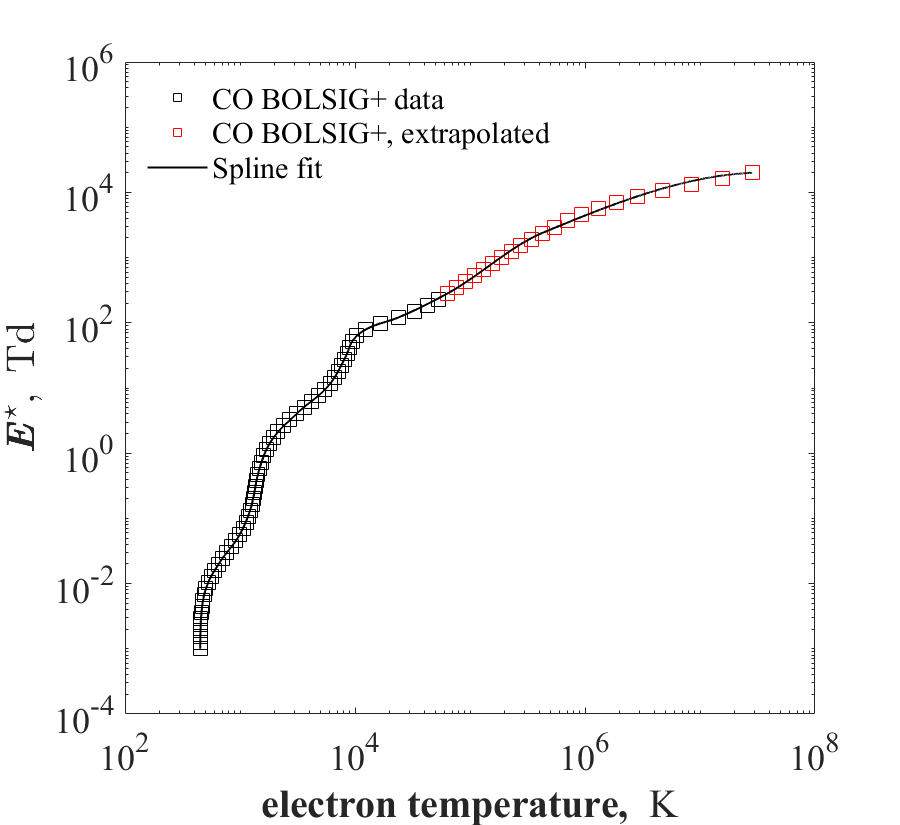
\includegraphics[width=0.99\linewidth, angle=0.0,scale=0.49]{electronimpact_figs/electronimpact_figureCO.png}}
\subfigure[]{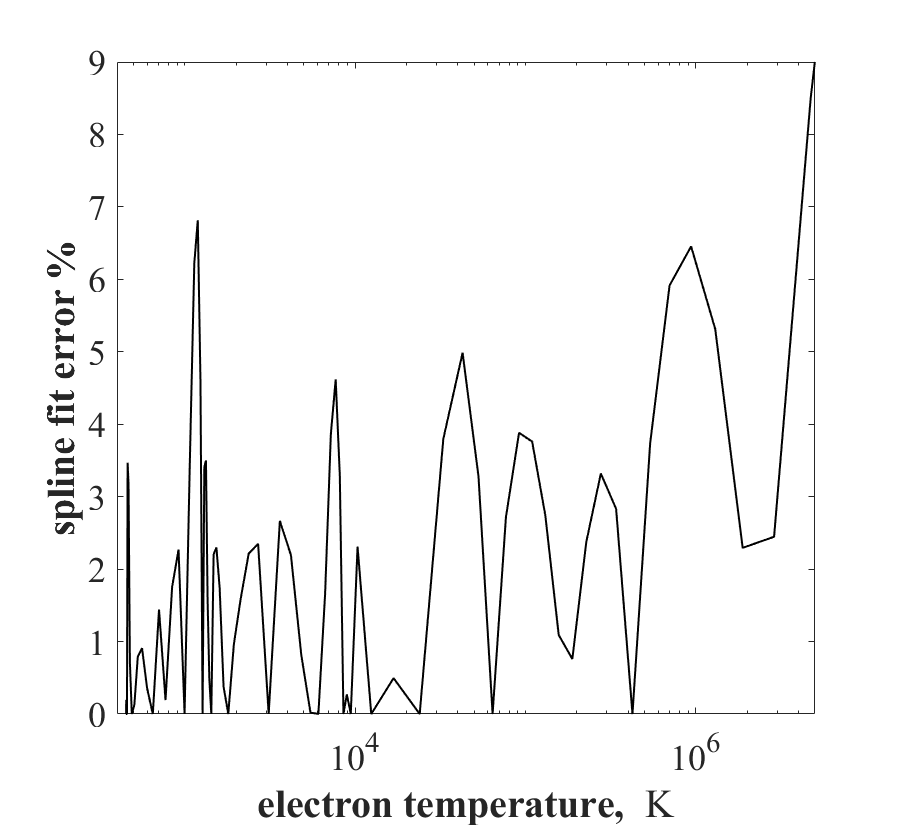
\includegraphics[width=0.99\linewidth, angle=0.0,scale=0.49]{electronimpact_figs/electronimpact_figureCO_error.png}}
\subfigure[]{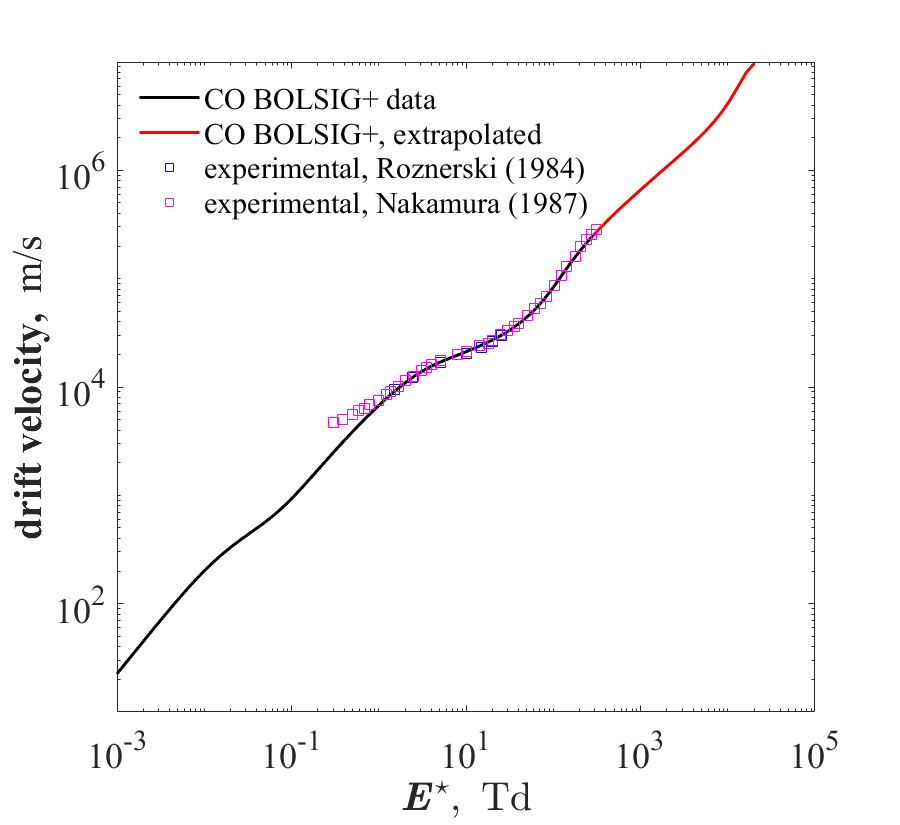
\includegraphics[width=0.99\linewidth, angle=0.0,scale=0.49]{electronimpact_figs/electronimpact_figureCO_drift.png}}
\caption{$E^\star$ results for $\rm CO$, showing (a) reduced electric field as a function of the electron temperature, b) error percentage when fitting a cubic spline through the data and (c) bulk drift velocity of electrons in carbon monoxide as a function of the reduced electric field. The electron impact cross-sectional data used in the BOLSIG+ calculation is sourced from the Morgan lxcat database. Experimental data points are taken from Fig. 6 of Ref.\ \cite{jop:1987:nakamura} and Fig. 3 of Ref.\ \cite{jop:1984:roznerski}.}
\label{fig:electronimpact_CO}
\end{figure}
%



\begin{table}[!htbp]
  \center\fontsizetable
  \begin{threeparttable}
    \tablecaption{Coordinates of control points for monotone cubic spline interpolation of electron impact processes\tnote{a}.}
    \label{tab:spline_tab}
    \fontsizetable
    \begin{tabular*}{\textwidth}{l@{\extracolsep{\fill}}lcll}
    \toprule
   No.~~ & Process ~& Variable & Spline control point coordinates  \\
        \midrule

        

  \multirow{2}{*}{1} &  \multirow{2}{*}{ $\rm e^- + N  $   } & ${\rm ln}~T_{\rm e}$  & \tiny      6.1322    6.2124    6.4474    7.5872    8.7256    9.2774    9.4778    9.5934   10.0915   11.1390   11.7497   13.5255   15.4249
 \\
  &  & ${\rm ln}~E^\star$     & \tiny -55.2620  -54.4162  -53.5703  -51.4558  -49.7641  -48.9182  -48.0721  -47.2264  -45.1117  -43.4205  -42.5745  -40.8824  -39.6301\\     
  \midrule  
      
  \multirow{2}{*}{2} &  \multirow{2}{*}{ $\rm e^- + O  $   } & ${\rm ln}~T_{\rm e}$  & \tiny    6.1395    6.2392    6.5051    7.6315    8.6771    9.1363    9.2668    9.3848    9.5799   10.1629   10.8830   11.2996   11.6030   12.4065   15.4249 \\
  &  & ${\rm ln}~E^\star$     & \tiny  -55.2620  -54.4162  -53.5703  -51.4558  -49.7641  -48.9182  -48.0721  -47.2264  -46.3806  -45.1117  -44.2660  -43.4205  -42.5745  -40.8824  -39.0042\\     
  \midrule    
  
  \multirow{2}{*}{3} &  \multirow{2}{*}{ $\rm e^- + N_2 $   } & ${\rm ln}~T_{\rm e}$  & \tiny          5.7836    6.0067    7.0566    9.0580    9.6956   10.0010   11.4313   11.9302   14.1582   15.4249
\\
  &  & ${\rm ln}~E^\star$     & \tiny       -51.8608  -51.0135  -49.5583  -46.7448  -44.4423  -43.7491  -42.3992  -41.6848  -39.5410  -38.7385
\\
  \midrule  
  
  \multirow{2}{*}{4} &  \multirow{2}{*}{ $\rm e^- + O_2  $   } & ${\rm ln}~T_{\rm e}$  & \tiny         6.1549    7.3930    8.6458    9.4545   10.2346   10.9063   11.1835   11.8793   12.6550   13.6691   14.3029   15.4249 \\ 

  &  & ${\rm ln}~E^\star$     & \tiny      -50.6569  -48.3543  -46.7448  -46.0517  -44.9531  -43.5718  -43.0406  -41.9779  -40.9153  -39.8524  -39.3210  -38.7385

  \\     
  \midrule  
  
  \multirow{2}{*}{5} &  \multirow{2}{*}{ $\rm e^- + NO  $   } & ${\rm ln}~T_{\rm e}$  & \tiny    4.6052    5.0387    5.7384    6.0438    6.9078    8.1163    8.3684    9.4004    9.9245   10.2589   11.3016   12.0194   13.1593   14.9141
 \\
  &  & ${\rm ln}~E^\star$     & \tiny    -53.3605  -52.4569  -51.1678  -50.6572  -49.3446  -45.9734  -45.3367  -44.6079  -44.2446  -43.7196  -42.4083  -41.3594  -40.0476  -38.7385
  \\     
  \midrule  
        
  \multirow{2}{*}{6} &  \multirow{2}{*}{ $\rm e^- + NH_3  $   } & ${\rm ln}~T_{\rm e}$  & \tiny 6.2086    6.2700    6.8003    8.8806   10.1453   10.3802   10.7743   11.9975   15.4249   \\
  
  &  & ${\rm ln}~E^\star$     & \tiny   -46.3062  -45.8896  -45.3691  -44.9524  -44.5359  -44.3277  -43.5990  -41.7243  -39.7238  \\
    \midrule  
  \multirow{2}{*}{7} &  \multirow{2}{*}{ $\rm e^- + NH_3$$(v)$   } & ${\rm ln}~T_{\rm e}$  & \tiny     6.1332    6.2103    6.4055    6.4643    6.5402    6.6125    7.0325    9.3651   10.5660   10.9750   12.5994   15.4249
  \\
  
  &  & ${\rm ln}~E^\star$     & \tiny     -49.7948  -49.0140  -48.0380  -47.2567  -46.4757  -46.0852  -45.3041  -44.7183  -43.9374  -43.1563  -41.2036  -39.4587
  \\  
  
    \midrule  
  \multirow{2}{*}{8} &  \multirow{2}{*}{ $\rm e^- + C_2 H_4$   } & ${\rm ln}~T_{\rm e}$  & \tiny         6.1098    6.1121    6.1155    6.1188    6.1487    6.2766    6.4902    7.5115    9.9324   11.1645   12.6660   15.4249
  \\
  
  &  & ${\rm ln}~E^\star$     & \tiny       -55.2620  -54.4110  -53.9853  -53.7725  -52.9212  -50.7933  -48.6652  -46.5372  -44.4092  -42.2812  -40.1532  -38.4508
  \\  
  
    \midrule  
  \multirow{2}{*}{9} &  \multirow{2}{*}{ $\rm e^- + H_2 O$   } & ${\rm ln}~T_{\rm e}$  & \tiny         6.1101    6.1160    6.1517    6.4204    6.7792    7.5390    9.7639   10.9427   11.3091   12.7398   15.4249
  \\
  
  &  & ${\rm ln}~E^\star$     & \tiny      -49.3036  -48.2401  -47.1756  -45.6864  -45.0478  -44.6221  -44.1963  -43.5577  -42.9197  -40.7916  -38.8686
  \\  
  
  
    \midrule  
  \multirow{3}{*}{10} &  \multirow{3}{*}{ $\rm e^- + CO$   } & ${\rm ln}~T_{\rm e}$  & \tiny     6.1114    6.1124    6.1139    6.1203    6.1262    6.1912    6.4755    6.9046    7.1482    7.2660    7.4955    8.0413    8.7133    9.0518    9.1509    9.4277   10.0823   11.0675   12.9578   17.1610

  \\
  
  &  & ${\rm ln}~E^\star$     & \tiny  -55.2620  -55.0494  -54.8361  -54.4110  -54.1980  -53.3469  -52.2829  -51.2188  -50.1549  -49.0908  -48.0271  -46.9628  -45.8990  

  \\  
  
&  &   & \tiny -44.8347  -44.4092  -43.9836  -43.5577  -42.7067  -40.5790  -38.4508 \\
                       
    \bottomrule
    \end{tabular*}
\begin{tablenotes}
\item[{a}] Notation and units: $T_{\rm e}$ is the electron temperature in Kelvin and $E^\star$ is the reduced electric field in units of V$\rm ~m^2$.
\end{tablenotes}
   \end{threeparttable}
\end{table}
